%%%%%%%%%%%%%%%%%%%%%%%%%%%%%%%%%%%%%%%%%
% Masters/Doctoral Thesis 
% LaTeX Template
% Version 1.42 (19/1/14)
%
% This template has been downloaded from:
% http://www.latextemplates.com
%
% Original authors:
% Steven Gunn 
% http://users.ecs.soton.ac.uk/srg/softwaretools/document/templates/
% and
% Sunil Patel
% http://www.sunilpatel.co.uk/thesis-template/
%
% License:
% CC BY-NC-SA 3.0 (http://creativecommons.org/licenses/by-nc-sa/3.0/)
%
% Note:
% Make sure to edit document variables in the Thesis.cls file
%
%%%%%%%%%%%%%%%%%%%%%%%%%%%%%%%%%%%%%%%%%

%----------------------------------------------------------------------------------------
%	PACKAGES AND OTHER DOCUMENT CONFIGURATIONS
%----------------------------------------------------------------------------------------

\documentclass[11pt, a4paper, oneside]{Thesis} % Paper size, default font size and one-sided paper

\graphicspath{{Pictures/}} % Specifies the directory where pictures are stored

\usepackage[square, numbers, comma, sort&compress]{natbib} % Use the natbib reference package - read up on this to edit the reference style; if you want text (e.g. Smith et al., 2012) for the in-text references (instead of numbers), remove 'numbers' 
\hypersetup{urlcolor=blue, colorlinks=true} % Colors hyperlinks in blue - change to black if annoying
\title{\ttitle} % Defines the thesis title - don't touch this

\begin{document}

\frontmatter % Use roman page numbering style (i, ii, iii, iv...) for the pre-content pages

\setstretch{1.3} % Line spacing of 1.3

% Define the page headers using the FancyHdr package and set up for one-sided printing
\fancyhead{} % Clears all page headers and footers
\rhead{\thepage} % Sets the right side header to show the page number
\lhead{} % Clears the left side page header

\pagestyle{fancy} % Finally, use the "fancy" page style to implement the FancyHdr headers

\newcommand{\HRule}{\rule{\linewidth}{0.5mm}} % New command to make the lines in the title page

% PDF meta-data
\hypersetup{pdftitle={\ttitle}}
\hypersetup{pdfsubject=\subjectname}
\hypersetup{pdfauthor=\authornames}
\hypersetup{pdfkeywords=\keywordnames}

%----------------------------------------------------------------------------------------
%	TITLE PAGE
%----------------------------------------------------------------------------------------

\begin{titlepage}
\begin{center}

\textsc{\LARGE \univname}\\[1.5cm] % University name
\textsc{\Large Doctoral Thesis}\\[0.5cm] % Thesis type

\HRule \\[0.4cm] % Horizontal line
{\huge \bfseries \ttitle}\\[0.4cm] % Thesis title
\HRule \\[1.5cm] % Horizontal line
 
\begin{minipage}{0.4\textwidth}
\begin{flushleft} \large
\emph{Author:}\\
\href{http://www.johnsmith.com}{\authornames} % Author name - remove the \href bracket to remove the link
\end{flushleft}
\end{minipage}
\begin{minipage}{0.4\textwidth}
\begin{flushright} \large
\emph{Supervisor:} \\
\href{http://www.jamessmith.com}{\supname} % Supervisor name - remove the \href bracket to remove the link  
\end{flushright}
\end{minipage}\\[3cm]
 
\large \textit{A thesis submitted in fulfilment of the requirements\\ for the degree of \degreename}\\[0.3cm] % University requirement text
\textit{in the}\\[0.4cm]
\groupname\\\deptname\\[2cm] % Research group name and department name
 
{\large \today}\\[4cm] % Date
%\includegraphics{Logo} % University/department logo - uncomment to place it
 
\vfill
\end{center}

\end{titlepage}

%----------------------------------------------------------------------------------------
%	DECLARATION PAGE
%	Your institution may give you a different text to place here
%----------------------------------------------------------------------------------------

\Declaration{

\addtocontents{toc}{\vspace{1em}} % Add a gap in the Contents, for aesthetics

I, \authornames, declare that this thesis titled, '\ttitle' and the work presented in it are my own. I confirm that:

\begin{itemize} 
\item[\tiny{$\blacksquare$}] This work was done wholly or mainly while in candidature for a research degree at this University.
\item[\tiny{$\blacksquare$}] Where any part of this thesis has previously been submitted for a degree or any other qualification at this University or any other institution, this has been clearly stated.
\item[\tiny{$\blacksquare$}] Where I have consulted the published work of others, this is always clearly attributed.
\item[\tiny{$\blacksquare$}] Where I have quoted from the work of others, the source is always given. With the exception of such quotations, this thesis is entirely my own work.
\item[\tiny{$\blacksquare$}] I have acknowledged all main sources of help.
\item[\tiny{$\blacksquare$}] Where the thesis is based on work done by myself jointly with others, I have made clear exactly what was done by others and what I have contributed myself.\\
\end{itemize}
 
Signed:\\
\rule[1em]{25em}{0.5pt} % This prints a line for the signature
 
Date:\\
\rule[1em]{25em}{0.5pt} % This prints a line to write the date
}

\clearpage % Start a new page

%----------------------------------------------------------------------------------------
%	QUOTATION PAGE
%----------------------------------------------------------------------------------------

\pagestyle{empty} % No headers or footers for the following pages

\null\vfill % Add some space to move the quote down the page a bit

\textit{``Thanks to my solid academic training, today I can write hundreds of words on virtually any topic without possessing a shred of information, which is how I got a good job in journalism."}

\begin{flushright}
Dave Barry
\end{flushright}

\vfill\vfill\vfill\vfill\vfill\vfill\null % Add some space at the bottom to position the quote just right

\clearpage % Start a new page

%----------------------------------------------------------------------------------------
%	ABSTRACT PAGE
%----------------------------------------------------------------------------------------

\addtotoc{Abstract} % Add the "Abstract" page entry to the Contents

\abstract{\addtocontents{toc}{\vspace{1em}} % Add a gap in the Contents, for aesthetics

The Thesis Abstract is written here (and usually kept to just this page). The page is kept centered vertically so can expand into the blank space above the title too\ldots
}

\clearpage % Start a new page

%----------------------------------------------------------------------------------------
%	ACKNOWLEDGEMENTS
%----------------------------------------------------------------------------------------

\setstretch{1.3} % Reset the line-spacing to 1.3 for body text (if it has changed)

\acknowledgements{\addtocontents{toc}{\vspace{1em}} % Add a gap in the Contents, for aesthetics

The acknowledgements and the people to thank go here, don't forget to include your project advisor\ldots
}
\clearpage % Start a new page

%----------------------------------------------------------------------------------------
%	LIST OF CONTENTS/FIGURES/TABLES PAGES
%----------------------------------------------------------------------------------------

\pagestyle{fancy} % The page style headers have been "empty" all this time, now use the "fancy" headers as defined before to bring them back

\lhead{\emph{Contents}} % Set the left side page header to "Contents"
\tableofcontents % Write out the Table of Contents

\lhead{\emph{List of Figures}} % Set the left side page header to "List of Figures"
\listoffigures % Write out the List of Figures

\lhead{\emph{List of Tables}} % Set the left side page header to "List of Tables"
\listoftables % Write out the List of Tables

%----------------------------------------------------------------------------------------
%	ABBREVIATIONS
%----------------------------------------------------------------------------------------

\clearpage % Start a new page

\setstretch{1.5} % Set the line spacing to 1.5, this makes the following tables easier to read

\lhead{\emph{Abbreviations}} % Set the left side page header to "Abbreviations"
\listofsymbols{ll} % Include a list of Abbreviations (a table of two columns)
{
\textbf{LAH} & \textbf{L}ist \textbf{A}bbreviations \textbf{H}ere \\
%\textbf{Acronym} & \textbf{W}hat (it) \textbf{S}tands \textbf{F}or \\
}

%----------------------------------------------------------------------------------------
%	PHYSICAL CONSTANTS/OTHER DEFINITIONS
%----------------------------------------------------------------------------------------

\clearpage % Start a new page

\lhead{\emph{Physical Constants}} % Set the left side page header to "Physical Constants"

\listofconstants{lrcl} % Include a list of Physical Constants (a four column table)
{
Speed of Light & $c$ & $=$ & $2.997\ 924\ 58\times10^{8}\ \mbox{ms}^{-\mbox{s}}$ (exact)\\
% Constant Name & Symbol & = & Constant Value (with units) \\
}

%----------------------------------------------------------------------------------------
%	SYMBOLS
%----------------------------------------------------------------------------------------

\clearpage % Start a new page

\lhead{\emph{Symbols}} % Set the left side page header to "Symbols"

\listofnomenclature{lll} % Include a list of Symbols (a three column table)
{
$a$ & distance & m \\
$P$ & power & W (Js$^{-1}$) \\
% Symbol & Name & Unit \\

& & \\ % Gap to separate the Roman symbols from the Greek

$\omega$ & angular frequency & rads$^{-1}$ \\
% Symbol & Name & Unit \\
}

%----------------------------------------------------------------------------------------
%	DEDICATION
%----------------------------------------------------------------------------------------

\setstretch{1.3} % Return the line spacing back to 1.3

\pagestyle{empty} % Page style needs to be empty for this page

\dedicatory{For/Dedicated to/To my\ldots} % Dedication text

\addtocontents{toc}{\vspace{2em}} % Add a gap in the Contents, for aesthetics

%----------------------------------------------------------------------------------------
%	THESIS CONTENT - CHAPTERS
%----------------------------------------------------------------------------------------

\mainmatter % Begin numeric (1,2,3...) page numbering

\pagestyle{fancy} % Return the page headers back to the "fancy" style

% Include the chapters of the thesis as separate files from the Chapters folder
% Uncomment the lines as you write the chapters

% Chapter 1

\chapter{Introduzione} % Main chapter title

\label{Chapter1} % For referencing the chapter elsewhere, use \ref{Chapter1} 

\lhead{Capitolo 1. \emph{Introduzione}} % This is for the header on each page - perhaps a shortened title

La prima parte di questa relazione vuole presentare al lettore il contesto di lavoro dell'azienda ospitante il progetto di stage.

%----------------------------------------------------------------------------------------


\section{Azienda}
\begin{figure}[h]\centering  

\includegraphics[scale=0.38]{/workspace/1911_up/Dropbox/thesis/Figures/logo_sanmarco.png}
\caption[Logo Aziendale]{Logo Aziendale}
\label{pic-a}
\end{figure}

Nata negli anni '80 come software house specializzata negli applicativi per aziende manifatturiere, SanMarco Informatica (http://www.sanmarcoinformatica.it/) è una società italiana che mira principalmente allo sviluppo di software gestionali. Con l'aumento esponenziale della telefonia mobile e dell'internet in mobilità (attraverso smartphone), è stata resa evidente la necessità di ripensare al modo in cui interfacciarsi con il cliente Business. Oltre alle transizioni B2B (Business-to-Business), SanMarco valuta la creazione di particolari software, commissionati da clienti già acquisiti, che possa permettere al pubblico di conoscere meglio il prodotto venduto. 

Nello specifico il progetto aziendale richiedeva la creazione di un software per un cliente del settore oculistico, attraverso il quale un potenziale cliente potesse:

\begin{itemize}
\item Scegliere gli occhiali preferiti da una lista presente sullo schermo dello smarthphone
\item Provare attraverso un feedback visivo, in realtà aumentata, tali occhiali
\item Condividere attraverso i Social Networks una fotografia eventualmente scattata
\end{itemize}

Dato che l'azienda ospitante non possedeva un background in tali ambiti (rilevamento facciale ed integrazione social su piattaforme mobile native), è nata l'esigenza di effettuare uno studio di fattibilità. Nonostante la novità e la natura del progetto, sono state utilizzate tecnologie alternative ma sono state comunque adottate le fasi di sviluppo tipicamente seguite dall'azienda.

\section{Progetto}

\section{Processi Interni}

Le fasi di sviluppo di progetto seguite dall'azienda sono, per ordine:
\begin{itemize}

\item Coordinamento e Riunioni. In questa fase vengono pianificate tutte le attività necessarie allo
svolgimento del progetto.
\item Analisi dei requisiti. L'output dell'attività di analisi è un documento in cui vengono racchiusi
tutti i requisiti funzionali, qualitativi, prestazionali e dichiarativi dei quali il prodotto finale
dovrà garantirne il soddisfacimento. Il documento serve da input per la fase di progettazione
\item Progettazione. Nella fase di progettazione si definiscono le specifiche tecniche delle funzionalità
da realizzare. Il risultato di questa fase è il documento di Specifiche Tecniche di Progettazione
\item Stadio esecutivo del progetto con il quale si realizzano i moduli software previsti
\item Test funzionali e di sistema. I test funzionali hanno lo scopo di verificare che i moduli realizzati
durante la fase di codifica rispettino quanto fissato dai requisiti iniziali. Il test di sistema valida
il prodotto nella sua interezza
\item Collaudo con il cliente. Si tratta di un test di sistema effettuato su un ambiente del cliente
e con dati di prova forniti dallo stesso. L'output di questa attività è un verbale che racconta
l'esito del collaudo
\item Documentazione di prodotto. Questa fase prevede la stesura dei Manuali di Prodotto relativi
al software realizzato
L'output di ogni fase viene verificato e, se conforme agli standard qualitativi dell'azienda, approvato.
Altrimenti dovranno essere indicate delle misure correttive per i problemi individuati

\end{itemize}

%----------------------------------------------------------------------------------------


%% Chapter 1

\chapter{Progetto Aziendale} % Main chapter title

\label{Chapter2} % For referencing the chapter elsewhere, use \ref{Chapter1} 

\lhead{Capitolo 2. \emph{Progetto Aziendale}} % This is for the header on each page - perhaps a shortened title

%----------------------------------------------------------------------------------------
Come annunciato nel precedente capitolo, cardini di questo progetto sono il rilevamento del volto (e delle sue parti) e la condivisione di contenuti attraverso i Social Networks.
A seguire verranno fornite informazioni di carattere formativo su tali punti.

\section{Rilevamento facciale}

Il rilevamento facciale è una tecnica di intelligenza artificiale utilizzata per verificare la presenza di un volto a partire da una o più immagini che lo ritraggono.\\
Si può affermare che si tratti di un riconoscimento di pattern (dove il pattern da riconoscere è un volto umano), che avviene mediante tecniche di elaborazione di immagini digitali. Viene utilizzato in biometria, per sistemi di videosorveglianza ma anche per usi generici, come ad esempio per l'autofocus nelle odierne fotocamere digitali. 

Negli anni sono stati creati numerosi algoritmi a tale scopo.
Alcuni di essi usano analizzano:

\begin{itemize}
\item il colore della pelle (nelle immagini a colori)
\item il movimento (nei video)
\item la forma della testa
\item combinazione delle caratteristiche sopra elencate
\end{itemize}

Comunque si scelga l'algoritmo, le problematiche che si incontrano nella ricerca della presenza di volti sono:

\begin{itemize}
\item Qualità dell'immagine non adeguata (sgranata, non a fuoco, risoluzione insufficiente)
\item Condizione d'illuminazione non ottimale (sottoesposizione o sovraesposizione eccessiva)
\item Espressioni facciali non campionate (quando i volti presenti assumono espressioni non presenti nel template di confronto)
\item Variazione della "messa in posa"
\item Variazioni d'aspetto del volto (ad esempio i tratti di un volto di una persona di origine asiatica saranno notevolmente diversi da quelli di una persona di origine europea)
\end{itemize}

\subsection{Machine Learning}

Data la complessità del problema è difficile creare una soluzione unica che abbia un'accuratezza soddisfacente. Una delle strade migliori è costruire un classificatore e collezionare una grande database di esempi di classificazione, creare una funzione di classificazione parametrizzata e successivamente ottimizzarla. Questa metodologia è definita machine learning. 

Ne è un esempio la tecnica di rilevamento facciale sviluppato da Paul Viola e Michael Jones che utilizza le cosidette \textit{diagonal features} all'interno di un classificatore chiamato \textit{Haar}. Questo classificatore utilizza un algoritmo di tipo AdaBoost (Adaptive Boosting) ma lo organizza come una cascata di nodi dove ogni nodo è un un multialbero di classificatori AdaBoost istruiti per avere un altissimo rate di rilevamento. Tale "istruzione" deriva dal training dato dalle Haar-like features ricavate da immagini digitali. Queste immagini contengono volti normalizzati (scalati e traslati) correttamente per un rapporto 1:6000 rispetto al totale delle immagini utilizzate (le rimanenti non rappresentano facce).


\begin{figure}[H]\centering  
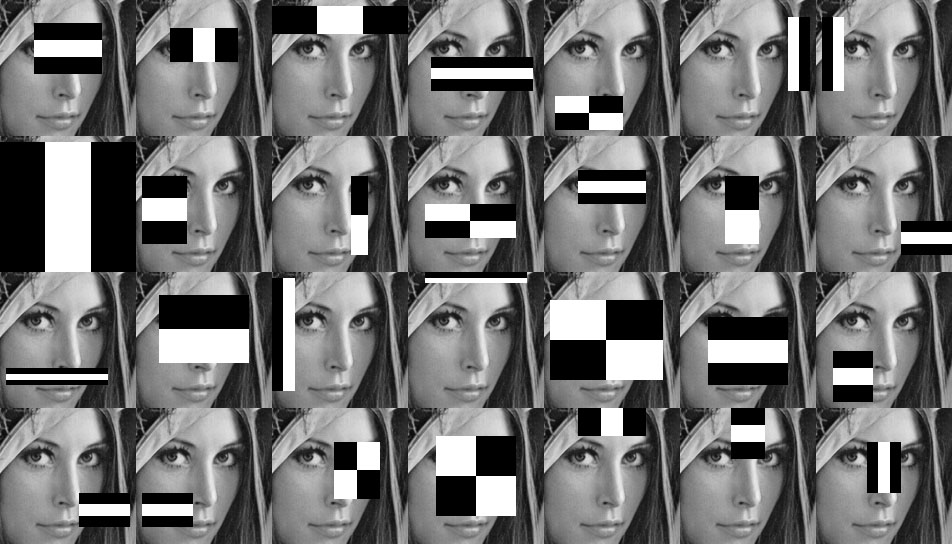
\includegraphics[scale=0.35]{/home/nicgen/Scrivania/thesis/Figures/feature.jpg}
\caption[Esempio di utilizzo delle features]{Esempio di utilizzo delle features}
\label{pic-a}
\end{figure}

Ad ogni nodo raggiunto, un singolo risultato negativo porta alla terminazione del processo, e l'algoritmo esce dichiarando di non aver trovato volti all'interno dell'immagine data. Ogni nodo deve rispondere nella seguente forma: 

Il valore \textit{k} trovato per la feature \textit{f} è sotto o sopra a una certa soglia \textit{S}? 
\begin{itemize}
\item \textbf{Si}, quindi la regione di interesse considerata è un volto.
\item \textbf{No}, altrimenti.
\end{itemize}

Tipicamente i nodi sono ordinati dal meno al più complesso (i primi nodi sono generalmente molto semplici). In tal modo si può ridurre notevolmente il costo computazionale di rilevamento del volto, perché le regioni dell'immagine che non lo contengono terminano subito nei primissimi nodi se non al primo.

\begin{figure}[H]\centering  
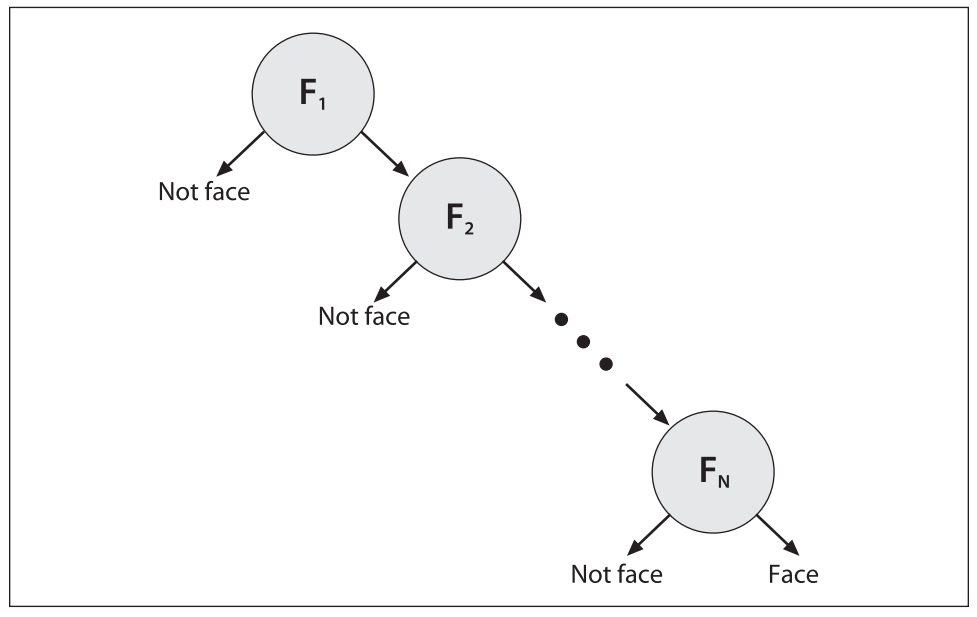
\includegraphics[scale=0.3]{/home/nicgen/Scrivania/thesis/Figures/boosted.png}
\caption[Binary Rejection cascade]{Binary Rejection cascade}
\label{pic-a}
\end{figure}

Tale algoritmo permette di raggiungere un alto tasso di accuratezza, infatti in media il numero di falsi negativi è inferiore all' 1 per cento mentre il numero di falsi positivi si attesta sotto al 40 per cento.

\section{Condivisione Social}

I siti di reti sociali (social network sites) sono servizi web che tipicamente permettono di:
\begin{itemize}
\item Creare un profilo pubblico o semi-pubblico all'interno di un sistema vincolato
\item Ottenere una lista di contatti associata a tale profilo
\item Condividere sul proprio profilo o su quello altrui contenuti testuali o multimediali
\end{itemize}

Una relazione sociale costruita sulla base di un interesse è totalmente differente da una costruita a partire da reti sociali virtuali, in cui il legame nasce a prescindere dalla presenza di interessi comuni o informazioni da condividere.
L'idea alla base di quest'ultima rete è che ogni utente possa avere uno scambio bidirezionale di informazioni con altri utenti. In un'era in cui buona parte della popolazione mondiale utilizza tale strumento di comunicazione, è quindi spesso fondamentale integrare al software funzionalità di condivisione.

\begin{figure}[H]\centering  
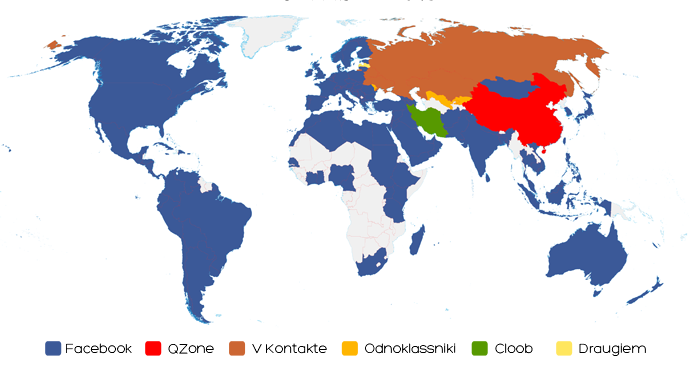
\includegraphics[scale=0.7]{/home/nicgen/Scrivania/thesis/Figures/snetwork.png}
\caption[Mappa distribuzione Social Networks]{Mappa distribuzione Social Networks, Dicembre 2013}
\label{pic-a}
\end{figure}

A seguito di un'analisi sul target di mercato, l'Azienda ha deciso di utilizzare il Social Network Facebook che, come in figura, è tra i più utilizzati a livello globale. Inoltre Facebook fornisce agli sviluppatori delle \textit{SDK} che permettono di ottenere una grande mole di informazioni sull'utente che installa l'applicazione e sull'ambiente attraverso cui comunica (numeri di telefono, e-mail, nominativi dei conoscenti, fotografie, etc.). Tali informazioni, se gestite correttamente, possono essere fondamentali per comprendere se il prodotto venga effettivamente utilizzato dal mercato per cui l'applicazione è stata concepita.

%----------------------------------------------------------------------------------------

\section{Obiettivi}

L'esigenza primaria dell'azienda ospitante era quello di creare una libreria di appoggio per il rilevamento facciale che rispettasse gli standard funzionali e qualitativi Android. Tale esigenza era dettata dal fatto di voler applicare tale funzionalità ad una famiglia di prodotti molto diversificata come ad esempio:

\begin{itemize}
\item \textbf{Oculistica per il cliente} come già definito nell'introduzione di tale documento
\item \textbf{Intrattenimento}
\begin{itemize}
\item \textbf{Videogiochi} 
utilizzo del riconoscimento facciale per variare l'esperienza d'utilizzo del videogioco a seconda della posizione e della quantità di volti presenti di fronte al dispositivo
\item \textbf{Generico}
utilizzo del riconoscimento facciale per applicazioni ludiche generiche, come ad esempio il face-swapping
\end{itemize}
\end{itemize}  

Secondaria ma non meno importante (obbligatoria) è la creazione di una libreria che permetta una facile instaurazione e comunicazione verso il social network Facebook per la condivisione di foto o di altri contenuti multimediali.

%----------------------------------------------------------------------------------------

\section{Aspettative}

L'azienda si aspettava che l'obiettivo principale venisse raggiunto.

%----------------------------------------------------------------------------------------

\section{Vincoli}

Non sono stati imposti vincoli particolari per quanto riguarda lo svolgimento del progetto di stage.
I vincoli imposti sono:
\begin{itemize}
 	\item Utilizzare il linguaggio Java per l'implementazione del prototipo
 	\item Utilizzare IntelliJ IDEA e nello specifico l'SDK Android che fornisce le librerie API e gli strumenti di sviluppo necessarie al build, test e debug delle applicazioni
 	\item Garantire flessibilità ed estensibilità futura del prototipo
 	\item Garantire il funzionamento per le versioni Android uguali o superiori alla v2.3 (Gingerbread)
 	\item Fornire documentazione adeguata sul prototipo implementato
 	\item Utilizzare il repository SVN aziendale per il versionamento del progetto
 	\item Rispettare la timeline preventivata
\end{itemize}

Nonostante il progetto sia inteso come studio di fattibilità e realizzazione di un prototipo, si dovrà cercare di rispettare le seguenti guidelines Android e Facebook:
\begin{itemize}
\item L'applicazione deve richiedere il minor numero di permessi possibile
\item L'applicazione non deve richiedere permessi di accedere a dati sensibili
\item L'applicazione deve supportare entrambi i possibili orientamenti del dispositivo
\item L'applicazione non deve lasciare servizi attivi quando questa è in background, a meno che questi non siano vitali per essa
\item L'applicazione deve preservare e ripristinare correttamente lo stato al fine di evitare perdite di dati accidentali:
\begin{itemize}
\item Se l'applicazione è ripristinata dallo switch di applicazioni recenti o da uno stato di sleep, deve ritornare esattamente com'era prima di esser stata messa in background
\item Se si riceve un input OnBackPressed, deve venire chiesto all'utente se è nelle sue intenzioni salvare i contenuti della sessione corrente ed uscire
\end{itemize}
\item L'applicazione non deve crashare o funzionare in maniera anormale a seconda del dispositivo
\end{itemize}


%----------------------------------------------------------------------------------------

 
%% Chapter 1

1.1\chapter{Pianificazione ed Analisi} % Main chapter title

\label{Capitolo 3} % For referencing the chapter elsewhere, use \ref{Chapter1} 

\lhead{Capitolo 3. \emph{Attività di stage}} % This is for the header on each page - perhaps a shortened title

%----------------------------------------------------------------------------------------

\section{Pianificazione}

Viene di seguito riportato un diagramma di Gantt riassuntivo della pianificazione
del lavoro nel periodo di stage. Come si può vedere le ore sono state suddivise secondo
2 obiettivi, che rappresentano parti di sistema indipendenti che verranno sviluppate
in maniera autonoma.\\

\begin{figure}[h]\centering  
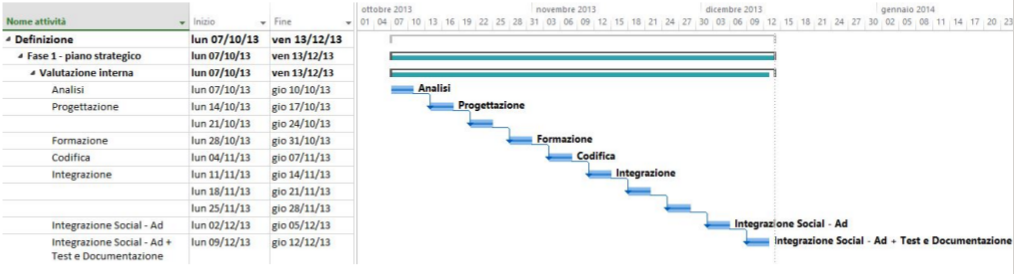
\includegraphics[scale=0.37]{/home/nicgen/Scrivania/thesis/Figures/tempo.png}
\caption[Pianificazione temporale]{Pianificazione temporale definita}
\label{pic-a}
\end{figure}

Il modello di ciclo di vita prescelto può essere paragonabile allo scrum: viene infatti preferito rispetto alla rigidità dei modelli più classici, in
quanto permetteva lo sviluppo continuo dei vari incrementi e la possibilità di mostrare
passo per passo i risultati ottenuti. Per chiarezza si riporta una breve descrizione degli
obiettivi presenti nel piano di lavoro che verranno maggiormente approfonditi nelle
sezioni successive:

\textbf{Obiettivo 1}: Studiare la fattibilità prestazionale di un software di rivelamento facciale e delle sue parti su un dispositivo mobile.

\textbf{Obiettivo 2}: Creazione di una libreria di appoggio ad OpenCV che renda di facile utilizzo il rilevamento facciale e delle parti presenti.

\textbf{Obiettivo 3}: Creazione di una libreria che permetta una facile condivisione dei contenuti multimediali eventualmente creati verso il social network Facebook.


%----------------------------------------------------------------------------------------

\section{Analisi}

In seguito allo studio del dominio applicativo effettuato durante le prime settimane di stage e alle spiegazioni del tutor aziendale sono stati individuati i requisiti del prototipo richiesto.
Dal momento che si tratta di un prototipo che dovrà essere alla base di una famiglia di prodotti, esso non sarà indipendente dall input umano ma dovrà garantire la flessibilità ed espandibilità necessaria.

Di seguito vengono riportati i casi d'uso principali individuati.

\subsection{Casi d'uso}

In questa sezione verranno elencati i casi d'uso del sistema che `e oggetto dello stage.
Dato che l'applicazione è stata pensata per rispondere solo alle azioni di un utente l'unico attore che prenderemo in
considerazione è l'utente utilizzatore. Per ogni caso d'uso verranno riportate:

\begin{itemize}
\item  \textit{Descrizione}: contenuto del caso d'uso
\item  \textit{Flusso principale degli eventi}
\item  \textit{Precondizioni}: asserzioni che sono valide prima dell'effettiva esecuzione del
caso d'uso
\item  \textit{Postcondizione}: asserzioni che sono valide dopo l'esecuzione del caso d'uso
\item  \textit{Postcondizione alternativa}: eventuali scenari alternativi che differiscono dal normale flusso del caso d'uso
\end{itemize}
Ogni caso d'uso ha un identificativo stile UCx dove x indica una posizione gerarchica.
Ogni caso d'uso è posizionato all'interno della gerarchia che parte dal caso d'uso più generale UC1 (radice dell'albero). Per ogni caso d'uso figlio valgono ovviamente le precondizioni del padre. Per chiarezza si definiscono gli acronimi per i termini RealTime (RT) e Static (S) per definire la duplice funzione dell'applicazione.

\subsubsection{UC1: Principale (RT)}

\textbf{\textit{Descrizione:}} L'utente ha avviato il programma, che risulta quindi pronto a rispondere agli eventuali input utente. L'utente può decidere lo Sprite da utilizzare.

\textbf{\textit{Flusso principale degli eventi:}} 

\begin{itemize}
\item L'utente può avviare il rilevamento del volto di parti facciali predefinite (UC1.1)
\item L'utente può calibrare la Camera (UC1.2)
\item L'utente può attivare la funzione di rilevamento di orientamento del volto (UC1.3)
\item L'utente può scegliere lo Sprite da utilizzare da una lista a schermo (UC1.4)
\end{itemize}

\textbf{\textit{Precondizione:}} L'applicazione è avviata e funzionante.


\begin{figure}[H]\centering  
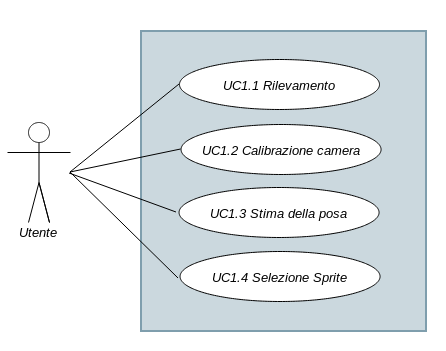
\includegraphics[scale=0.6]{/home/nicgen/Scrivania/thesis/Figures/uc1.png}
\caption[UC1 - Sistema]{UC1 - Sistema}
\label{pic-a}
\end{figure}


\subsubsection{UC2: Principale (S)}

\textbf{\textit{Descrizione:}} L'utente ha avviato il programma, che risulta quindi pronto a rispondere agli eventuali input utente. L'utente può decidere lo Sprite da utilizzare.

\textbf{\textit{Flusso principale degli eventi:}} 

\begin{itemize}
\item L'utente carica una foto dal dispositivo verso l'applicazione (UC2.1)
\item L'utente richiede la funzione di rilevamento del volto (UC2.2)
\item L'utente può scegliere lo Sprite da utilizzare da una lista a schermo (condiviso con UC2.3)
\end{itemize}

\textbf{\textit{Precondizione:}} L'applicazione è avviata e funzionante.

\begin{figure}[H]\centering  
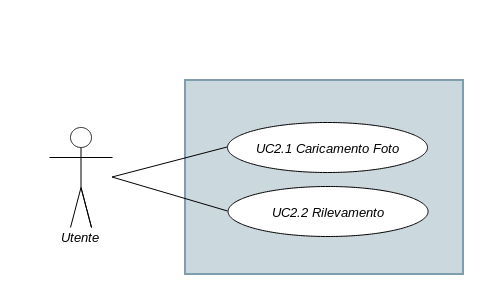
\includegraphics[scale=0.6]{/home/nicgen/Scrivania/thesis/Figures/uc2.png}
\caption[UC2 - Sistema]{UC2 - Sistema}
\label{pic-a}
\end{figure}


\subsubsection{UC3: Secondario}

\textbf{\textit{Descrizione:}} L'utente ha avviato il programma, ha scattato una foto in modalità dinamica o statica.

\textbf{\textit{Flusso principale degli eventi:}} 

\begin{itemize}
\item L'utente può ridimensionare la foto ottenuta in base a formati predefiniti (UC3.1)
\item L'utente può condividere la foto ottenuta verso applicazioni di messaggistica interne grazie al lancio di un Intent (UC3.2)
\item L'utente può effettuare il Login sulla piattaforma Facebook e condividere la foto su quest ultimo (UC3.3)
\end{itemize}

\textbf{\textit{Precondizione:}} L'applicazione è avviata e funzionante.

\begin{figure}[H]\centering  
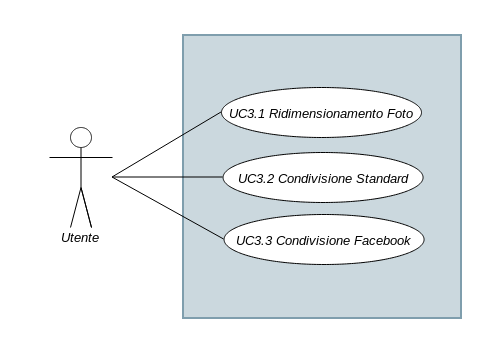
\includegraphics[scale=0.6]{/home/nicgen/Scrivania/thesis/Figures/uc3.png}
\caption[UC3 - Sistema]{UC3 - Sistema}
\label{pic-a}
\end{figure}


\subsubsection{UC1.1: (RT)::Rilevamento}

\textbf{\textit{Descrizione:}} L'utente può avviare il rilevamento del volto di parti facciali predefinite. L'applicazione reagisce con la creazione di templates che verranno successivamente riutilizzati per il tentativo di match sui frames successivi.


\textbf{\textit{Precondizione:}} L'applicazione è avviata e funzionante.
\textbf{\textit{Postcondizione:}} L'applicazione rileva gli eventuali volti presenti e le feature indicate.



\subsubsection{UC1.2: (RT)::Calibrazione Camera}

\textbf{\textit{Descrizione:}} 

\textbf{\textit{Flusso principale degli eventi:}} 

\begin{itemize}
\item L'utente può selezionare una camera (UC1.2.1)
\item L'utente può selezionare il tipo di elaborazione della camera (UC1.2.2)
\item L'utente può modificare la risoluzione del frame in ingresso (UC1.2.3)
\item L'utente può modificare la profondità di campionamento (distanza minima e massima su cui effettuare lo scan) (UC1.2.4)
\item L'utente può modificare il numero minimo di campionamenti sotto il quale il volto non viene riconosciuto come valido (UC1.2.5)
\item L'utente può abilitare/disabilitare lo scan delle parti facciali in tempo reale (UC1.2.6)
\item L'utente può abilitare/disabilitare la modalità alto contrasto e/o monocromatica (UC1.2.7)
\end{itemize}

\textbf{\textit{Precondizione:}} L'applicazione è avviata e funzionante. Inoltre l'utente ha espresso la volontà di utilizzare tale funzione attraverso la pressione di un bottone presente all'interno dell'interfaccia grafica.

\begin{figure}[H]\centering  
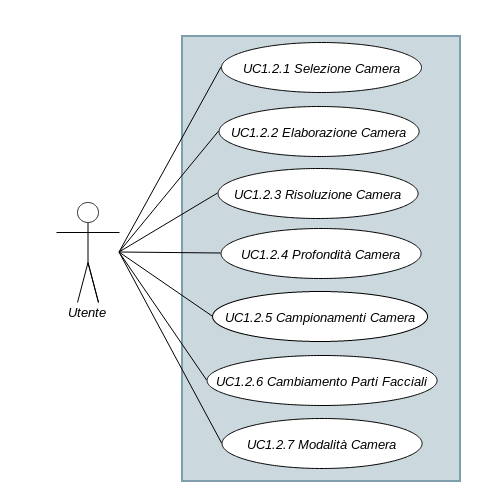
\includegraphics[scale=0.6]{/home/nicgen/Scrivania/thesis/Figures/uc12.png}
\caption[UC1.2 - Calibrazione camera]{UC1.2 - Calibrazione camera}
\end{figure}

\subsubsection{UC1.3: (RT)::Orientamento Volto}

\textbf{\textit{Descrizione:}} L'utente deve poter avviare la funzionalità che permette la triangolazione delle parti occhi-bocca per capire l'orientamento del volto in base alle fattezze dei triangolo individuato

\textbf{\textit{Postcondizione:}} L'applicazione rileverà in tempo reale l'orientamento del volto della persona rispetto alla camera grazie alla triangolazione delle parti occhi-bocca.


\subsubsection{UC1.4: (RT)::Selezione Sprite}

\textbf{\textit{Descrizione:}} L'utente può decidere quale tra i possibili Sprites utilizzare, da sovrapporre al volto individuato.

\textbf{\textit{Flusso principale degli eventi:}} 

\begin{itemize}
\item Caricamento all'interno di una ListView della lista di oggetti di tipo Sprite (UC1.4.1)
\item Selezione dello Sprite desiderato (UC1.4.2)
\item Effettiva renderizzazione dello Sprite che sarà posto in overlay su ogni fotogramma (UC1.4.3)
\end{itemize}

\textbf{\textit{Precondizione:}} L'applicazione è avviata e funzionante. Inoltre l'utente ha espresso la volontà di utilizzare tale funzione attraverso la pressione di un bottone presente all'interno dell'interfaccia grafica.

\begin{figure}[H]\centering  
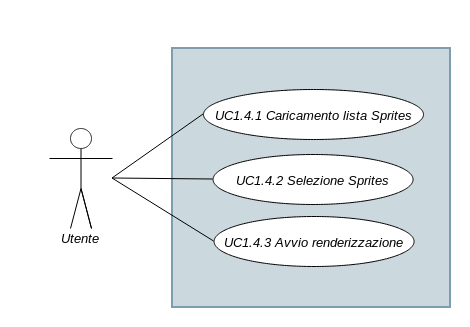
\includegraphics[scale=0.6]{/home/nicgen/Scrivania/thesis/Figures/uc14.png}
\caption[UC1.4 - Selezione Sprite]{UC3.3 - Selezione Sprite}
\label{pic-a}
\end{figure}

\subsubsection{UC2.1: (S)::Caricamento Foto}

\textbf{\textit{Descrizione:}} L'utente sceglie attraverso l'utilizzo di una galleria proprietaria di Android la foto da caricare.

\textbf{\textit{Postcondizione:}} L'applicazione carica al suo interno una foto proveniente dallo storage dello smartphone e la tiene in memoria.


\subsubsection{UC2.2: (S)::Rilevamento}

\textbf{\textit{Descrizione:}} L'utente può avviare il rilevamento del volto di parti facciali predefinite. L'applicazione reagisce con la creazione di un template del volto rilevato.


\textbf{\textit{Precondizione:}} L'applicazione è avviata e funzionante.
\textbf{\textit{Postcondizione:}} L'applicazione rileva gli eventuali volti presenti e le feature indicate.

\subsubsection{UC2.3: (S)::Selezione Sprite}

\textbf{\textit{Descrizione:}} L'utente può decidere quale tra i possibili Sprites utilizzare, da sovrapporre al volto individuato.

\textbf{\textit{Flusso principale degli eventi:}} 

\begin{itemize}
\item Caricamento all'interno di una ListView della lista di oggetti di tipo Sprite (UC1.4.1)
\item Selezione dello Sprite desiderato (UC1.4.2)
\item Effettiva renderizzazione dello Sprite che sarà posto in overlay su ogni fotogramma (UC1.4.3)
\end{itemize}

\textbf{\textit{Precondizione:}} L'applicazione è avviata e funzionante.

\subsubsection{UC3.1: Secondario::Ridimensionamento frame}

\textbf{\textit{Descrizione:}} L'utente può ridimensionare la foto ottenuta scegliendo tra formati predefiniti.

\textbf{\textit{Postcondizione:}} L'applicazione ridimensiona l'immagine in base alla dimensione definita dall'utente.


\subsubsection{UC3.2: Secondario::Condivisione Interna}

\textbf{\textit{Descrizione:}} L'utente può condividere la foto ottenuta verso applicazioni di messaggistica

\textbf{\textit{Flusso principale degli eventi:}} 

\begin{itemize}
\item L'utente deve poter esprimere il suo intento cliccando su un tasto presente all'interno dell'interfaccia grafica (UC3.2.1)
\item L'applicazione deve esporre i mezzi attraverso i quali il contenuto multimediale può essere condiviso (UC3.2.2)
\item L'applicazione condivide il contenuto multimediale in seguito alla selezione dell'utente (UC3.2.3)
\end{itemize}

\textbf{\textit{Precondizione:}} L'applicazione è avviata e funzionante.


\begin{figure}[H]\centering  
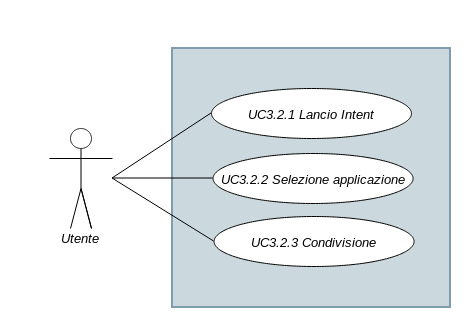
\includegraphics[scale=0.6]{/home/nicgen/Scrivania/thesis/Figures/uc32.png}
\caption[UC3.2 - Condivisione Interna]{UC3.2 - Condivisione Interna}
\label{pic-a}
\end{figure}

\subsubsection{UC3.3: Secondario::Facebook}

\textbf{\textit{Descrizione:}} L'utente ha avviato il programma, ha scattato una foto in modalità dinamica o statica.

\textbf{\textit{Flusso principale degli eventi:}} 

\begin{itemize}
\item L'utente può effettuare il login su facebook. (UC3.3.1)
\item L'utente può inserire un messaggio da allegare alla foto. (UC3.3.2)
\item L'utente può condividere tale contenuto sulla propria "bacheca" o su quella di altri conoscenti. (UC3.3.3)
\end{itemize}

\textbf{\textit{Postcondizione alternativa:}} L'applicazione è avviata e funzionante.


\begin{figure}[H]\centering  
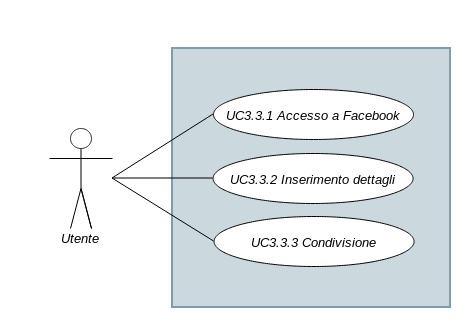
\includegraphics[scale=0.6]{/home/nicgen/Scrivania/thesis/Figures/uc33.png}
\caption[UC3.3 - Condivisione Facebook]{UC3.3 - Condivisione Facebook}
\label{pic-a}
\end{figure}

\subsubsection{UC1.2.1: (RT)::Calibrazione Camera::Selezione Camera}

\textbf{\textit{Descrizione:}} L'utente ha la possibilità di selezionare tra le camere presenti all'interno del dispositivo,se disponibili. 

\textbf{\textit{Postcondizione:}} L'applicazione ha accesso all'utilizzo della camera.

\textbf{\textit{Postcondizione alternativa:}} L'applicazione non ha accesso all'utilizzo della camera.

\subsubsection{UC1.2.2: (RT)::Calibrazione Camera::Elaborazione Camera}

\textbf{\textit{Descrizione:}} L'utente ha la possibilità di selezionare che tipo di camera utilizzare (Nativa OpenCV o Android) 

\textbf{\textit{Postcondizione:}} L'applicazione utilizzerà da quel momento il tipo di camera input selezionato

\subsubsection{UC1.2.3: (RT)::Calibrazione Camera::Risoluzione Camera}

\textbf{\textit{Descrizione:}} L'utente ha la possibilità di selezionare la risoluzione alla quale scalare il frame in ingresso.

\textbf{\textit{Postcondizione:}} L'applicazione scalerà ogni frame in ingresso alla risoluzione indicata dall'utente, mantenendo l'aspect ratio.

\subsubsection{UC1.2.4: (RT)::Calibrazione Camera::Profondità Camera}

\textbf{\textit{Descrizione:}}  L'utente ha la possibilità di selezionare la dimensione minima e massima (range operativo) secondo le quali il campionamento va effettuato.

\textbf{\textit{Postcondizione:}} L'applicazione effettuerà il campionamento nel range definito.

\subsubsection{UC1.2.5: (RT)::Calibrazione Camera::Campionamenti Camera}

\textbf{\textit{Descrizione:}} L'utente ha la possibilità di selezionare il numero di campionamenti al di sotto del quale il volto rilevato viene valutato come non valido e quindi scartato.

\textbf{\textit{Postcondizione:}} L'applicazione effettua lo scan del frame basandosi sul numero di campionamenti settato dall'utente, al di sotto del quale il volto rilevato viene valutato come non valido e quindi scartato. 

\subsubsection{UC1.2.6: (RT)::Calibrazione Camera::Parti Facciali}

\textbf{\textit{Descrizione:}} L'utente ha la possibilità di selezionare quali parti facciali abilitare.

\textbf{\textit{Postcondizione:}} L'applicazione eseguirà la ricerca di tutte le parti impostate dall'utente.

\subsubsection{UC1.2.7: (RT)::Calibrazione Camera::Modalità Camera}

\textbf{\textit{Descrizione:}} L'utente ha la possibilità di decidere se il frame in ingresso deve essere riconvertito in un immagine monocromatica e/o se esso debba subire un'elaborazione atta ad elevarne il contrasto.

\textbf{\textit{Postcondizione:}} L'applicazione applicherà la modalità definita.

\subsubsection{UC1.4.1: (RT)::Selezione Sprite::Caricamento Sprites}

\textbf{\textit{Descrizione:}} L'applicazione deve permettere su richiesta il caricamento su una ListView della lista di oggetti di tipo Sprite.

\textbf{\textit{Postcondizione:}} L'applicazione popola, attraverso l'utilizzo di un adapter, la ListView presente all'interno dell'interfaccia grafica.

\subsubsection{UC1.4.2: (RT)::Selezione Sprite::Selezione Sprites}

\textbf{\textit{Descrizione:}} L'applicazione deve permettere la selezione dello Sprite desiderato.

\textbf{\textit{Postcondizione:}} L'applicazione terrà in memoria lo Sprite selezionato, pronto per l'effettivo render.

\subsubsection{UC1.4.3: (RT)::Selezione Sprite::Visione Sprites}

\textbf{\textit{Descrizione:}} L'applicazione deve permettere l'effettiva renderizzazione dello Sprite che sarà posto in overlay su ogni fotogramma.

\textbf{\textit{Postcondizione:}} L'applicazione renderizza lo sprite in overlay, su ogni fotogramma, in corrispondenza del volto rilevato.

\subsubsection{UC3.2.1: Secondario::Condivisione Interna::Intent }

\textbf{\textit{Descrizione:}} L'utente deve poter esprimere il suo intento cliccando su un tasto presente all'interno dell'interfaccia grafica.

\textbf{\textit{Postcondizione:}} L'applicazione prepara l'adapter per il caricamento delle applicazioni di condivisione e popola la ListView.

\subsubsection{UC3.2.2: Secondario::Condivisione Interna::Selezione}

\textbf{\textit{Descrizione:}} L'applicazione deve esporre i mezzi attraverso i quali il contenuto multimediale può essere condiviso.

\textbf{\textit{Postcondizione:}} L'applicazione rende visibile a schermo gli le applicazioni disponibili.

\subsubsection{UC3.2.3: Secondario::Condivisione Interna::Condivisione}

\textbf{\textit{Descrizione:}} L'applicazione deve rispondere alla scelta dell'utente di utilizzare quella particolare applicazione per la condivisione del contenuto multimediale.

\textbf{\textit{Postcondizione:}} L'applicazione condivide il contenuto multimediale in seguito alla selezione dell'utente.

\subsubsection{UC3.3.1: Secondario::Facebook::Login}

\textbf{\textit{Descrizione:}} L'utente può inoltrare la richiesta di accesso alla piattaforma Facebook attraverso l'uso di un bottone presente all'interno dell'interfaccia grafica.

\textbf{\textit{Postcondizione:}} L'utente ha accesso alla piattaforma con i dovuti permessi. La classe si impegna di mantenere in memoria la sessione attiva 

\textbf{\textit{Postcondizione alternativa:}} L'utente non ha accesso alla piattaforma e viene invitato a controllare i dati di accesso.

\subsubsection{UC3.3.2: Secondario::Facebook::Messaggio}

\textbf{\textit{Descrizione:}} L'utente può scegliere se aggiungere un messaggio testuale alla foto .

\textbf{\textit{Postcondizione:}} L'utente ha inserito un messaggio testuale che sarà preso in consegna al momento dell'eventuale invio dei contenuti.

\textbf{\textit{Postcondizione alternativa:}} L'utente non ha inserito un messaggio testuale.

\subsubsection{UC3.3.3: Secondario::Facebook::Condivisione}

\textbf{\textit{Descrizione:}} L'utente può scegliere se la destinazione della foto sarà la propria "bacheca" o quella di altri conoscenti.

\textbf{\textit{Postcondizione:}} L'utente carica con successo il contenuto.

\textbf{\textit{Postcondizione alternativa:}} Il contenuto non viene caricato per problemi di connessione verso la piattaforma.



\subsection{Associazione Requisiti-Casi d'uso}

La classificazione dei requisiti sarà seguirà il formalismo:
\begin{center}
	\textbf{R\{TIPO\}\{RICHIESTA\}\{GERARCHIA\}}
\end{center}

Nello specifico:
\begin{itemize}
\item TIPO può essere:
	\begin{itemize}
		\item F, indica un requisito funzionale
		\item Q, indica un requisito di qualità
		\item V, indica un requisito di vincolo
	\end{itemize} 
\item IMPEGNO può essere:
	\begin{itemize}
		\item O, indica un requisito obbligatorio
		\item D, indica un requisito desiderabile
	\end{itemize} 
\item GERARCHIA: i requisiti sono organizzati gerarchicamente secondo una struttura ad albero. Se la complessità di un requisito viene ritenuta elevata, questo può essere diviso in sotto-requisiti.
\end{itemize}

A seguire i requisiti individuati:

\begin{center}
    \begin{longtable}{ | p{2cm} | p{7cm} | p{2cm} |}
    \hline
    Requisiti & Descrizione & Caso d'uso \\ \hline
    RFO1 &  L'applicazione deve permettere il rilevamento facciale in tempo reale su dispositivi mobili Android & UC1  \\ \hline 
    RFO1.1 &  L'utente può avviare il rilevamento del volto di parti facciali predefinite. L'applicazione reagisce con la creazione di templates che verranno successivamente riutilizzati per il tentativo di match sui frames successivi  & UC1.1 \\ \hline
    RFO1.2 &  L'applicazione deve permettere di calibrare la camera corrente  & UC1.2  \\ \hline 
    RFO1.2.1 &  L'applicazione deve permettere all'utente di selezionare la camera desiderata & UC1.2.1  \\ \hline
    RFO1.2.2 &  L'applicazione deve permettere all'utente di modificare il tipo di elaborazione della camera & UC1.2.2  \\ \hline
    RFO1.2.3 &  L'applicazione deve permettere all'utente di modificare la risoluzione del frame in ingresso & UC1.2.3  \\ \hline
    RFO1.2.4 &  L'applicazione deve permettere all'utente di modificare la profondità di campionamento (distanza minima e massima su cui effettuare lo scan) & UC1.2.4  \\ \hline
    RFO1.2.5 &  L'applicazione deve permettere all'utente di modificare il numero minimo di campionamenti sotto il quale il volto non viene riconosciuto come valido  & UC1.2.5  \\ \hline
    RFO1.2.6 &  L'applicazione deve permettere all'utente di abilitare di abilitare/disabilitare la ricerca delle parti in tempo reale  & UC1.2.6  \\ \hline
    RFO1.2.7 &  L'applicazione deve permettere all'utente di abilitare/disabilitare la modalità contrasto e/o monocromatica  & UC1.2.7  \\ \hline
    RFD1.3 &  L'applicazione deve permettere di cogliere l'orientamento dell'eventuale volto individuato & UC1.3 \\ \hline    
    RFD1.4 &  L'applicazione deve permettere di scegliere lo Sprite da utilizzare & UC1.4 \\ \hline
    RFO1.4.1 &  L'applicazione deve caricare una lista di Sprites, che saranno successivamente selezionabili dall'utente & UC1.4.1  \\ \hline
    RFO1.4.2 &  L'applicazione deve permettere all'utente di selezionare uno o più Sprites desiderati da una ListView presente all'interno dell'interfaccia grafica  & UC1.4.2  \\ \hline
    RFO1.4.3 &  L'applicazione deve poter renderizzare gli Sprites precedentemente selezionati & UC1.4.3  \\ \hline    
    RFO2 &  L'applicazione deve permettere di rilevare volti a partire da un immagine statica su dispositivi mobili Android & UC2  \\ \hline
    RFO2.1 &  L'applicazione deve permettere all'utente di caricare una foto dal proprio smartphone & UC2.1  \\ \hline 
    RFO2.2 &  L'applicazione deve permettere di avviare il rilevamento facciale & UC2.2 \\ \hline
    RFD2.3 &   L'applicazione deve permettere di scegliere uno o più Sprites da utilizzare  & UC2.3  \\ \hline 
    RFO3 &  L'applicazione deve permettere la condivisione di contenuti multimediali & UC3 \\ \hline
    RFD3.1 &  L'applicazione deve permettere di ridimensionare la foto scattata in base a formati predefiniti & UC3.1 \\ \hline
    RFD3.2 &  L'applicazione deve permettere di condividere la foto ottenuta verso applicazioni di messaggistica interne  & UC3.2 \\ \hline
    RFD3.2.1 &  L'applicazione deve fornire l'utente di un bottone attraverso il quale può esprimere il suo intento di condividere il contenuto  & UC3.2.1 \\ \hline
    RFD3.2.2 &  L'applicazione deve rispondere fornendo graficamente una risposta contenente i servizi di inoltro disponibili  & UC3.2.2 \\ \hline
    RFD3.2.3 &  L'applicazione deve condividere il contenuto multimediale attraverso il servizio selezionato  & UC3.2.3 \\ \hline    
    RFD3.3 &  L'applicazione deve permettere il login facebook e condividere la foto su quest ultimo  & UC3.3 \\ \hline
    RFD3.3.1 &  L'applicazione deve permettere l'inoltro di una richiesta di accesso verso i server Facebook ed il mantenimento della sessione attiva & UC3.3.1 \\ \hline
    RFD3.3.2 &  L'applicazione deve permettere l'inserimento di un testo da allegare alla foto & UC3.3.2 \\ \hline
    RFD3.3.3 &  L'applicazione deve permettere il caricamento della foto sulla piattaforma Facebook & UC3.3.3 \\ \hline
    RFD4 &  L'applicazione deve mantenere un framerate minimo di 15 fotogrammi al secondo & non mappabile \\ \hline
    \end{longtable}
    
    \textbf{Appunto RFD4}: Un sistema è scalabile se può essere adattato a diversi contesti con forti differenze di complessità senza che questo richieda la riprogettazione dello stesso sistema. Si richiede che le prestazioni di un sistema possano essere aumentate "semplicemente" fornendo al sistema stesso maggiori risorse di calcolo. Nello specifico si richiede che il sistema mantenga il framerate minimo indicato per gli smartphone Android aventi sistema operativo uguale o successivo ad \textit{HoneyComb}.
\end{center}


%\chapter{Progettazione} % Main chapter title

\label{Capitolo4} % For referencing the chapter elsewhere, use \ref{Chapter1} 

\lhead{Capitolo 4. \emph{Progettazione}} % This is for the header on each page - perhaps a shortened title

Molto spesso, non si progetta una struttura che reagisca in maniera elastica ma coerente alle modifiche.
Ad aggravare la situazione, i cambiamenti effettuati non sempre sono documentati per cui le specifiche non vengono aggiornate e ciò rende i cambiamenti futuri difficili da compiere. Conscio di tale realtà, si è cercato di progettare il sistema tenendo in mente le possibili evoluzioni.

\section{Architettura}



Il concetto di MVC sul sistema operativo Android è piuttosto vago. Infatti la filosofia delle API è incentrata sulla derivazione piuttosto che sulla composizione, il che rende anche difficile fare dei test accurati.

Le linee guida di Google per gli sviluppatori indicano che è necessario:

\begin{itemize}
\item Definire la UI (User Interface) in diversi XML in base alla risoluzione e all'hardware
\item Definire le risorse in altri XML
\item Estendere classi come ListActivity,TabActivity e utilizzare i sopracitati XML attraverso l'uso di inflaters
\item Creare le classi desiderate per la Business Logic
\end{itemize}

Vengono quindi definiti per ordine di peso i seguenti 7 Packages:

\begin{itemize}
\item Activity
\item Service
\item DataModel
\item Core
\item Social
\item Util
\item Adapter
\end{itemize}

\subsection{Package Activity}

Le activity sono uno dei 4 elementi di base che vanno a costituire un'applicazione:

\begin{itemize}
\item Activity
\item Broadcast Intent Receiver
\item Service
\item Content Provider
\end{itemize}

La classe Activity è uno degli elementi centrali di ogni applicazione Android. L'Activity è un concetto legato allo sviluppo delle interfacce grafiche: normalmente una Activity rappresenta una singola schermata della nostra applicazione. Le applicazioni possono definire una o più Activity per trattare diverse fasi del software: ogni Activity è responsabile del salvataggio del proprio stato in modo da poterlo ristabilire successivamente come parte del ciclo di vita dell'applicazione.
Ci può essere solo una Activity attiva per volta, quindi una sola Activity per volta può essere in “primo piano” nello stesso tempo: una che in un determinato momento non si trova nello stato attivo e quindi non si trova in foreground potrebbe essere terminata dal sistema operativo ad esempio perché la memoria diventa insufficiente. Questo significa che ogni applicazione Android può cambiare lo stato in ogni momento e deve essere pronta ad essere interrotta e chiusa in ogni istante.

A seguire il modello di ciclo di vita di una Activity:

\begin{figure}[h]\centering  
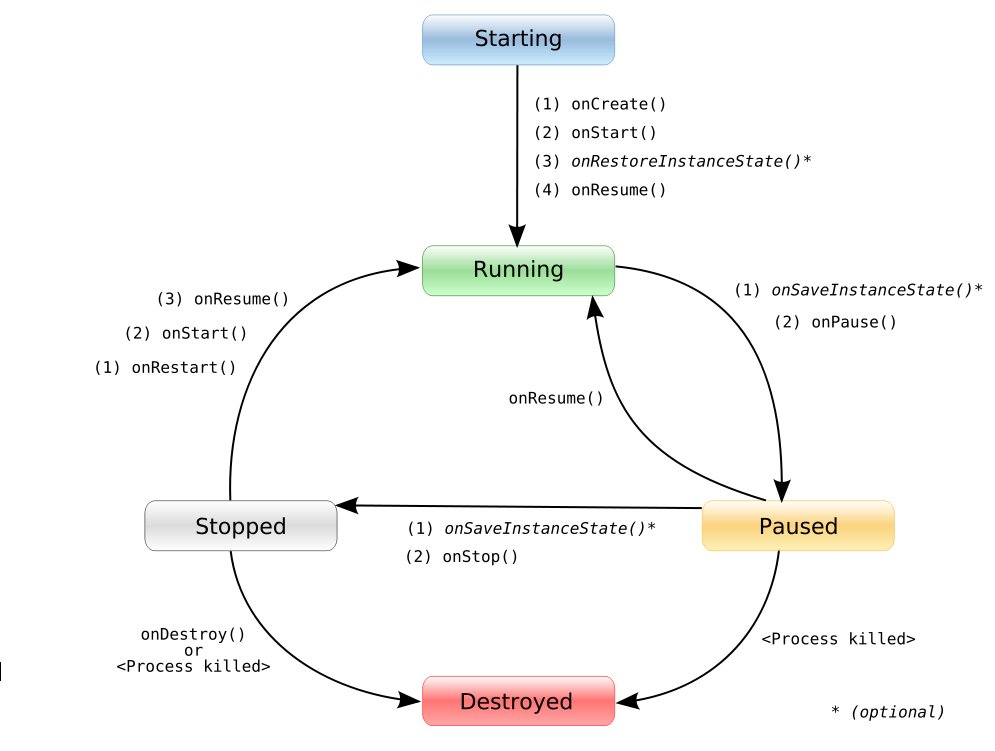
\includegraphics[scale=0.38]{/home/nicgen/Scrivania/thesis/Figures/ciclovitaattivita.jpg}
\caption[Long caption]{Caption}
\label{pic-a}
\end{figure}

L'attività richiesta in tale progetto consiste in una view che permetta di mandare a schermo i fotogrammi registrati dalla fotocamera ed altre informazioni d'uso. Essa deve inoltre registrare tutte le informazioni utili quali gli input utente.

Vengono quindi definite le seguenti Activity:
\begin{itemize}


\item \textbf{Activity::FaceDetectionActivity}

\textit{Estende:} Activity.

\textit{Implementa:} CvCameraViewListener2.

\textit{Descrizione ed utilizzo:} Attività poggiata su un subclassing di una classe di OpenCV dedita al riconoscimento di oggetti. Consente il rilevamento facciale e deve permettere di riconoscere le parti facciali richieste. Deve permettere di ricavare l'orientamento del volto in base alle fattezze del triangolo descritto dalla giunzione tra occhi e bocca.

\item \textbf{Activity::StaticFaceDetectionActivity}

\textit{Estende:} Activity. 

\textit{Descrizione ed utilizzo:} Simile a FaceDetectionActivity, ma la sua funzione è statica, ossia l'eventuale rilevamento si basa su immagini statiche inserite dall'utente (scattate al momento o caricate direttamente dallo smartphone).

\item \textbf{Activity::PhotoActivity}

\textit{Estende:} Activity.

\textit{Descrizione ed utilizzo:} Attività che permette di salvare l'eventuale fotografia scattata e di condividerla attraverso mail,servizi di messaggistica e Facebook.

\item \textbf{Activity::TutorialActivity}

\textit{Estende:} Activity.

\textit{Descrizione ed utilizzo:} Attività contenente un tutorial illustrativo che si prefigge di rendere chiaro l'utilizzo dell'applicazione.

\item \textbf{Activity::SplashScreenActivity}

\textit{Estende:} Activity.

\textit{Descrizione ed utilizzo :}Questa attività raccoglie semplicemente l'animazione del logo dell'azienda e deve permettere all'utente di scegliere se effettuare il login sul social network Facebook (opzionale per il proseguimento) ed inoltre permettere di accedere al programma previo accettazione dei termini di servizio.

\end{itemize}
\subsection{Package Service}

Un Service è un processo che lavora in background senza la diretta interazione con l'utente (un concetto molto simile al deamon in ambiente Unix). La classe Service viene utilizzata per creare componenti software che possono svolgere attività in modo “invisibile”, senza interfaccia utente. Utilizzando i Service è possibile gestire le nostre applicazioni e farle reagire ad eventi anche quando non sono in primo piano: un Service può essere avviato, fermato e controllato da altri componenti dell'applicazione, inclusi altri Service e Activity. Nello specifico tale strumento viene utilizzato per gestire eventuali chiamate al WebServer aziendale (richiesta di aggiornamento, sistema di notifiche).

Vengono così definite le classi:
\begin{itemize}


\item \textbf{Service::BootStartUpReceiver}

\textit{Estende:} BroadcastReceiver

\textit{Descrizione ed utilizzo:} Classe dedita esclusivamente all'avvio del Service indicato. E' possibile, tramite un particolare flag nel file \textit{Manifest.xml}, definire quando avviare tale servizio.

\item \textbf{Service::BackgroundService}

\textit{Estende:} Service. 

\textit{Descrizione ed utilizzo:} Classe che rappresenta il service dedito condivisione dei contenuti.
\end{itemize}

\subsection{Package Model}

Tale package è stato definito al fine di scindere il più possibile la parte puramente grafica dal modello.

Di seguito le classi definite:
\begin{itemize}

\item \textbf{Model::Data}

\textit{Estende:} nessuna classe.

\textit{Descrizione ed utilizzo:} Classe contenente i risultati degli input utente.

\item \textbf{Model::Sprite}

\textit{Estende:} nessuna classe.

\textit{Descrizione ed utilizzo:} Classe di diagnostica per il testing visuale dell'applicazione. Contiene i dati grezzi dei risultati ottenuti.

\end{itemize}
\subsection{Package Core}

\begin{itemize}
\item \textbf{Core::Camera}

\textit{Estende: JavaCameraView (OpenCV)}

\textit{Descrizione ed utilizzo:}permette la modifica dei parametri OpenCV a runtime quali risoluzione, profondità minima e massima di campionamento, numero di volti individuati necessari per la validazione, selezione della camera da utilizzare, etc.

\item \textbf{Core::Templates}

\textit{Estende:} nessuna classe. 

\textit{Descrizione ed utilizzo:} Classe contente funzioni che operano sui templates per il rilevamento del volto e delle parti richieste.
\end{itemize}
\subsection{Package Social}

Tale package contiene le classi:
\begin{itemize}
\item \textbf{Social::LoginSession}

\textit{Estende:} nessuna classe.

\textit{Descrizione ed utilizzo:} Classe che permette all'utente di effettuare l'accesso al social network Facebook e di mantenere la sessione di login attiva fino alla scadenza del token di validità.

\item \textbf{Social::Share}

\textit{Estende:} nessuna classe.

\textit{Descrizione ed utilizzo:} Classe adibita alla pubblicazione dei contenuti multimediali eventualmente creati.
\end{itemize}

\subsection{Package Utility}
Contiene le seguenti classi:

\begin{itemize}

\item \textbf{Utility::MatUtils}

\textit{Estende:} nessuna classe.

\textit{Descrizione ed utilizzo:} Classe generica per operazioni su oggetti appartenenti alla classe OpenCV Mat.

\item \textbf{Utility::Generics}

\textit{Estende:} nessuna classe.

\textit{Descrizione ed utilizzo:} Classe generica contenente principalmente funzioni statiche utilizzate per varie operazioni all'interno dell'applicazione.
\end{itemize}


\subsection{Package Adapter}
Contiene le seguenti classi:

\begin{itemize}

\item \textbf{Adapter::CustomAdapter}

\textit{Estende:} BaseAdapter.

\textit{Descrizione ed utilizzo:} Classe la cui instanza viene utilizzata per il caricamento di dati grezzi all'interno della ListView (utilizzata per la scelta degli Sprite o delle applicazioni disponibili per la condivisione).

\end{itemize}

\newpage

\section{Associazione Classi-Requisiti}

Di seguito viene indicata la mappatura Classi$\rightarrow$ Requisiti.

\begin{center}
    \begin{longtable}{| p{6cm} | p{2cm} |}
    \hline
    Classe & Requisito \\ \hline
     Activity::FaceDetectionActivity & RFO1.1  \\ \hline
     Core::Templates & RFO1.1 \\ \hline
     Utility::MatUtils & RFO1.1 \\ \hline
     Core::Camera & RFO1.2.1 \\ \hline
     Core::Camera & RFO1.2.2\\ \hline
     Core::Camera & RFO1.2.3  \\ \hline
     Core::Camera & RFO1.2.4 \\ \hline
     Core::Camera & RFO1.2.5\\ \hline
     Core::Camera & RFO1.2.6\\ \hline
     Core::Camera & RFO1.2.7 \\ \hline
     Activity::FaceDetectionActivity & RFD1.3 \\ \hline    
	 Model:Sprite & RFO1.4.1 \\ \hline
     Adapter::CustomAdapter & RFO1.4.2  \\ \hline
     Utility::Generics & RFO1.4.3 \\ \hline
     Activity::StaticFaceDetectionActivity & RFO2.1 \\ \hline
     Activity::StaticFaceDetectionActivity & RFO2.2\\ \hline
	 Model:Sprite & RFO2.3 \\ \hline
     Adapter::CustomAdapter & RFO2.3  \\ \hline
     Utility::MatUtils & RFD3.1 \\ \hline
     Activity::PhotoActivity & RFD3.2.1   \\ \hline
     Activity::PhotoActivity & RFD3.2.2  \\ \hline
     Service::BootStartUpReceiver & RFD3.2.2 \\ \hline
     Service::BackGroundService  & RFD3.2.2 \\ \hline
     Activity::PhotoActivity & RFD3.2.3 \\ \hline    
     Social::LoginSession & RFD3.3.1 \\ \hline
     Social::Share & RFD3.3.2 \\ \hline
     Social::Share & RFD3.3.3\\ \hline
     classe non mappata & RFD4  \\ \hline
     Activity::SplashScreenActivity & requisito non mappato  \\ \hline
     Activity::TutorialActivity & requisito non mappato  \\ \hline
    \end{longtable}
\end{center}

I requisiti non mappati corrispondono a richieste dell'azienda ospitante avvenute in corso d'opera, posteriori allo studio dell'architettura di sistema.

\section{Tecnologie utilizzate}

\subsection{Java}

Il linguaggio per applicazioni Android è in realtà un "dialetto" del linguaggio Java così come è diversa anche la virtual machine di runtime (Dalvik virtual machine anziché JVM).
In una normale applicazione Android non c'è un entry point (il classico metodo "main") da dove normalmente un programma comincia a caricare le sue parti software e avviarsi: tutto è pensato per essere un "componente" pilotato dagli eventi ("Event Driven") dell'hardware o di altri componenti. Questo paradigma fa sì che il programmatore sviluppi per ogni hardware delle routine il più possibile indipendenti. Un vantaggio è che il sistema operativo potrà ottimizzare le risorse, ad esempio rinunciando a caricare componenti (e hardware) non supportati o non prioritari perché inutilizzati.

\subsection{Android NDK}

L'NDK (Native Development Kit) è uno strumento che permette di implementare parte dell'applicazione usando codice scritto in linguaggio nativo come il C ed il C++. Per alcune applicazioni può essere utile in quanto si può riutilizzare le librerie scritte in tali linguaggi. L'uso di tale strumento non da però beneficio per la maggior parte delle applicazioni ed è da usare quindi con parsimonia (spesso l'aumento delle performance dovuto all'utilizzo di codice nativo non giustifica l'aumento di complessità). Tipicamente buoni candidati sono programmi che sono CPU-intensive che non allocano molta memoria come simulazioni fisiche ed analisi dei segnali. Nel caso specifico sono stati effettuati dei test per verificare se la quantità di chiamate verso la libreria C/C++ OpenCV giustifica tale strumento. Tale libreria è stata utilizzata per prototipi usa e getta ed è stata successivamente scartata per l'esiguo vantaggio prestazionale rispetto al notevole aumento della dimensione e complessità del codice.

\subsection{Android Studio}

Basato su IntelliJ IDEA, Android Studio è un ambiente di sviluppo integrato (IDE) specifico per la piattaforma Android. Esso fornisce strumenti molto potenti come lo smart editing, re-fattorizzazione del codice, layout editor, supporto a Gradle, supporto a Maven. Contiene al suo interno le SDK. Infatti le applicazioni di Android sono sviluppate all'interno di un framework, una struttura dati specifica che comprende un vasto set di strumenti di sviluppo come:

\begin{itemize}
\item Debugger
\item Dalvik Debug Monitor Server (DDMS)
\item Librerie Android
\item Emulatore basato su QEMU
\item Documentazione
\end{itemize}

\subsection{Android FD-Library}

All'interno delle SDK Android è presente una API per il riconoscimento facciale: Android.Media.FaceDetector. Questa classe permette, data un immagine, di trovare le eventuali facce presenti attraverso il semplice utilizzo del metodo findFaces(). Ogni istanza ritornata viene salvata in un array Faces[] e contiene:

\begin{itemize}
\item Valutazione se si tratta di un volto o meno 
\item Distanza tra gli occhi (numero di pixel)
\item Posizione (x,y) del punto medio situato tra i due occhi
\item Rotazioni di posa della faccia (x,y,z)
\end{itemize} 

A seguito di valutazioni e di un prototipo usa e getta si è però deciso di non utilizzare in quanto:

\begin{itemize}
\item Non ritorna il rettangolo che include con precisione la faccia

\item Non consente di utilizzare template a piacimento per la ricerca di parti specializzate (naso, occhi, orecchie, etc.)

\item Prestazioni buone per immagini singole, ma non adatta ad un applicazione real-time

\item Sono stati rilevati comportamenti evidentemente diversi a seconda del dispositivo utilizzato

\item Quantità non indifferente di bug riportata dalla comunità di sviluppatori Android
\end{itemize}

\subsection{OpenCV}

OpenCV è una libreria creata da Intel a scopi di commerciali e di ricerca. E' una libreria open e gratuita, e pertanto il suo codice può essere utilizzato nella sua interezza o in parte. Al momento della stesura di questo documento la versione più recente disponibile è la v2.4.7 specifica per dispositivi Android. Tale versione fornisce un wrapper Java alle librerie OpenCV che fornisce quasi tutte le fonzionalità core. Al fine di garantire il funzionamento di applicativi basati su questa libreria è però necessario installare sul dispositivo un software chiamato OpenCV Manager, che permette all'applicazione ottimizzazioni in base all'hardware presente.

Vi sono due modi d'utilizzo di questa libreria:

\begin{itemize}
\item \textbf{Ad alto livello}:  utilizzo esclusivo delle Java API. Facilità di sviluppo, ma non permette l'accesso completo alle libreria. Prestazioni minori a causa al gran numero di chiamate JNI (Java Native Interface) verso la libreria

\item \textbf{A basso livello}:  utilizzo dell'interfaccia nativa di openCV. Android permette infatti di eseguire chiamate a funzioni native, ciò significa che è possibile utilizzare l'interfaccia C++ di OpenCV. 
\end{itemize}
%----------------------------------------------------------------------------------------
\subsection{GenyMotion}

Genymotion è un emulatore Android alternativo disponibile per Windows, Mac e Linux. Verrà utilizzato al posto dell'emulatore proprietario di Android Studio per le sue doti velocistiche che permettono una non indifferente riduzione dei tempi di sviluppo.

\subsection{JTest}

JTest è una suite completa di strumenti per l'analisi statica del codice Java dal momento che fornisce molte informazioni sulle metriche (ne misura la complessità), individuando in esso i punti critici e facilitando così lo sviluppo del codice (che deve rispettare le norme assegnate). Facilita inoltre la review del codice, permette test d'unità e tracciamento di errori a tempo di esecuzione. E' lo strumento utilizzato dall'azienda ospitante lo stage, pertanto è di vincolo utilizzare tale sistema per il test dell'applicazione.


\subsection{Doxygen}

Doxygen è un tool per la generazione di documentazione di sorgenti di vario genere, compresi quelli Java. Esso si basa su un file di configurazione che contiene le numerose opzioni configurabili messe a disposizione per la generazione della documentazione. Inoltre supporta l'esportazione, tra le tante,
dei documenti sia in HTML che in LATEX. Nel progetto è stato utilizzato per la generazione di tutta la documentazione ottenibile dal codice in maniera automatica.

\subsection{Subversion}

Il sistema di controllo di versione utilizzato dall'azienda è SVN, pertanto è di vincolo utilizzare tale sistema per il versionamento dell'applicazione.


%----------------------------------------------------------------------------------------
\newpage
\section{Problematiche}

\subsection{Riduzione complessità}

Al fine di garantire un facile utilizzo della libreria Java OpenCV, sono state creati alcuni metodi con l'obbiettivo di suddividere il problema in sotto-problemi più semplici e facili da gestire e manutenere. L'intero rilevamento facciale e delle sue componenti viene gestito da un'unica funzione di dimensioni modeste:

\begin{lstlisting}
	public Mat onCameraFrame(CvCameraViewFrame inputFrame) {
		
		Mat equalizedGrayMat = MatUtils.equalize(inputFrame.gray());
		MatOfRect faces = new MatOfRect();
		
		mSelectedDetector.detectMultiScale(equalizedGrayMat, 
						faces, 
						mScaleFactor,
					        mMinNeighbors,
						mFlags, 
						mMinSize,
						mMaxsize);
						
		Rect[] facesArray = faces.toArray();

		for (int i = 0; i < facesArray.length; i++) {
			
			Rect r = facesArray[i];
			Rect eyearea = getEyesArea();
			Rect eyearea_right = getRightEyeRect(eyearea);
			Rect eyearea_left = getLeftEyeRect(eyearea);
			Rect nose_area = getNoseRect(getNoseROI(r, eyearea));
			Rect mouth_area = getMouthRect(getMouthROI(r, nose_area));

			if (mMust_Learn) {
				teplateER = create_new_template(mJavaDetectorEye, inputFrame.RGBA(), eyearea_right, 24, 1);
				teplateEL = create_new_template(mJavaDetectorEye, inputFrame.RGBA(), eyearea_left, 24, 1);
				teplateN = create_new_template(mJavaDetectorNose, inputFrame.RGBA(), nose_area, 24, 0);
				teplateM = create_new_template(mJavaDetectorMouth, inputFrame.RGBA(), mouth_area, 24, 0);
				.
				.
				//creazione di templates di interesse aggiuntivi
			} else {
			    match_feature(eyearea_right, teplateER, 1);
				match_feature(eyearea_left, teplateEL 1);
				match_feature(nose_area, teplateN, 2);
				match_feature(mouth_area, teplateM, 3); 
				.
				.
				//matching di templates di interesse aggiuntivi
			}
		}
\end{lstlisting}

Dove, sequenzialmente:
\begin{itemize}
\item il frame immagine in ingresso viene desaturato per ridurre la quantità di informazioni inoltrate, dal momento che l'algoritmo OpenCV lavora indipendentemente dai colori presenti. L'equalizzazione è invece necessaria per compensare le variazioni di luminosità nelle varie parti dell'immagine
\item la funzione \textit{detectMultiScale$(Mat ...)$} rileva i volti presenti e li immagazzina all'interno di un array (ne salva il rettangolo contenente il volto individuato)
\item per tutti gli elementi dell'array:
\begin{itemize}
\item ricava la regione d'interesse corrispondente alla feature da cercare (partendo dal presupposto che ogni feature facciale ha una posizione approssimabile statisticamente)
\item se viene richiesta la creazione di un template:
\begin{itemize}
\item crea un template grazie a un classificatore che lavora nella regione di interesse indicata in base al tipo della feature
\end{itemize}
\item altrimenti:
\begin{itemize}
\item esegue il template matching nella regione di interesse indicata
\end{itemize}
\end{itemize}
\end{itemize}

La prima funzione presa in analisi è \textit{redo\_template$(...)$} che trova la parte desiderata nella regione di interesse (ROI) indicata. 
Tale regione è stata ricavata da una stima statistica dell'altezza delle varie parti rispetto al volto ed è necessaria per ridurre al minimo il costo computazionale di ricerca delle singole parti. 

\begin{lstlisting}
    private void create_new_template(CascadeClassifier classificator, Mat source , Rect roi, boolean isEye) {
        Mat template = new Mat();
        Mat mROI = source.submat(roi);
        MatOfRect feature = new MatOfRect();
        Point iris = new Point();
        Rect feature_template = new Rect();
        classificator.detectMultiScale(mROI, feature, 1.15, 2,
                Objdetect.CASCADE_FIND_BIGGEST_OBJECT
                        | Objdetect.CASCADE_SCALE_IMAGE, new Size(30, 30),
                new Size());
 
        Rect[] eyesArray = feature.toArray();
        for (int i = 0; i < eyesArray.length;) {
            Rect e = eyesArray[i];
            e.x = area.x + e.x;
            e.y = area.y + e.y;
            Rect feature_rectangle = new Rect((int) e.tl().x,
                    (int) (e.tl().y + e.height * 0.4), (int) e.width,
                    (int) (e.height * 0.6));
            .
            .            
 \end{lstlisting} 
 
Di particolare valore è il metodo \textit{detectMultiScale(const Mat image, vector<Rect> objects, double scaleFactor, int minNeighbors, int flags, Size minSize, Size maxSize)} chiamato dal classificatore dove i parametri:
 \begin{itemize}
 \item \textit{scaleFactor}: indica di quanto la dimensione dell'immagine è ridotta ad ogni scaling. Si crea quindi una piramide di immagini in cui l'immagine in posizione k è di dimensioni inferiori all'immagine in posizione k-1. Maggiore sarà questo valore, minore sarà il costo computazionale ma lo sarà anche il rate di rilevamento.

\begin{figure}[h]\centering  
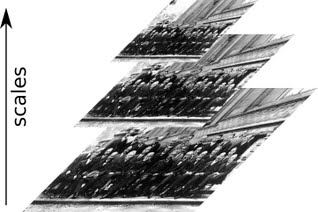
\includegraphics[scale=0.8]{/home/nicgen/Scrivania/thesis/Figures/pyramid.jpg}
\caption[Image Pyramid]{Image Pyramid}
\label{pic-a}
\end{figure} 

\item \textit{Image}: immagine di input, preferibilmente desaturata ed equalizzata.

\item \textit{objects}: vettore all'interno del quale saranno inseriti i rettangoli contenenti i volti individuati.

\item \textit{minNeighbors}: indica la qualità dei volti rilevati. Maggiore sarà tale parametro, maggiore sarà la precisione ma con il rischio che anche i volti corretti siano scartati.

\item \textit{flags}: indicano specifiche condizioni che il classificatore deve seguire (come ad esempio saltare alcune regioni o cercare l'oggetto di dimensioni massime).

\item \textit{minSize}: Dimensione minima degli oggetti, sotto la quale vengono ignorati.

\item \textit{maxSize}: Dimensione massima degli oggetti, oltre la quale vengono ignorati.
 
\end{itemize}
 
Nel caso l'input al metodo richieda di trovare l'occhio e in particolare la pupilla, riduco la regione di interesse e grazie alla funzione OpenCV \textit{Core.minMaxLoc(...)} è possibile trovare il punto più scuro dell'occhio (ossia la pupilla). 

Successivamente per questioni di verifica disegna sulla sottomatrice Mat il rettangolo contenente l'occhio e il cerchio contenente la pupilla.\\
         
\begin{lstlisting}    
                .    
                .
                mROI = source.submat(feature_rectangle);
                Mat vyrez = sourceRGBA.submat(feature_rectangle);
               
  	            Core.MinMaxLocResult darkPoint = Core.minMaxLoc(mROI);
            
 	            Core.circle(vyrez, darkPoint.minLoc, 2, new Scalar(255, 255, 255, 255), 2);
	            iris.x = darkPoint.minLoc.x + feature_rectangle.x;
 	            iris.y = darkPoint.minLoc.y + feature_rectangle.y;
	            feature_template = new Rect((int) iris.x - size / 2, (int) iris.y
	                    - size / 2, size, size);
	            Core.rectangle(sourceRGBA, feature_template.tl(), feature_template.br(),
 	                   new Scalar(255, 0, 0, 255), 2);
	            template = (source.submat(feature_template)).clone();
            }
            return template;
        }
        return template;
    }
\end{lstlisting}

Una volta creato il template, per i frame successivi verrà utilizzato \textit{match\_feature$(...)$} che appunto utilizza il template creato da \textit{create\_new\_template$(...)$}. 

Il template matching utilizzato per mezzo del metodo OpenCV \textit{$matchTemplate(...)$} non è basato su istogrammi ma è basato sul match di un template che viene fatto "scivolare" contro un'immagine di input.\\

\begin{figure}[H]\centering  
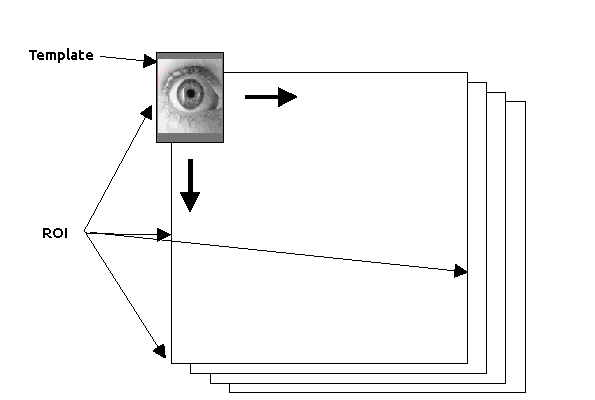
\includegraphics[scale=0.8]{/home/nicgen/Scrivania/thesis/Figures/slide.png}
\caption[Sliding Template Matching]{Sliding Template Matching}
\label{pic-a}
\end{figure}

\begin{lstlisting}
private void match_feature(Rect roi, Mat template, int type) {
        Point matchLoc;
        Mat ROI = mGray.submat(roi);
        int result_cols = mROI.cols() - template.cols() + 1;
        int result_rows = mROI.rows() - template.rows() + 1;
		
        Mat mResult = new Mat(result_cols, result_rows, CvType.CV_8U);
 
        Imgproc.matchTemplate(ROI, mTemplate, mResult,Imgproc.TM_CCORR_NORMED);
 
        Core.MinMaxLocResult mmres = Core.minMaxLoc(mResult);
		.
		.
		.
    }
\end{lstlisting}

Come si può vedere dalla funzione è stato utilizzato il metodo TM\_CCORR\_NORMED nella regione di interesse ROI. 

Utilizzando \textit{I} per denotare l'immagine in ingresso, \textit{T} per il template si definisce il metodo CV\_TM\_CCORR (Correlation matching method) come: 

\begin{figure}[H]\centering  
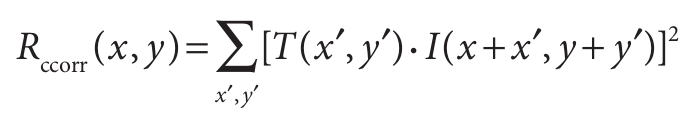
\includegraphics[scale=0.3]{/home/nicgen/Scrivania/thesis/Figures/rcor.png}
\caption[Correlation matching method formula]{Correlation matching method formula}
\label{pic-a}
\end{figure}

Dal momento che il template viene moltiplicato contro l'immagine, un match perfetto risulterà grande mentre un match cattivo sarà molto piccolo e tendente a 0.

Di tale metodo ne esiste una versione normalizzata che è utile perchè può ridurre gli effetti di differenze di luce tra l'immagine in ingresso ed il template utilizzato. Il coefficiente di normalizzazione viene definito come:

\begin{figure}[H]\centering  
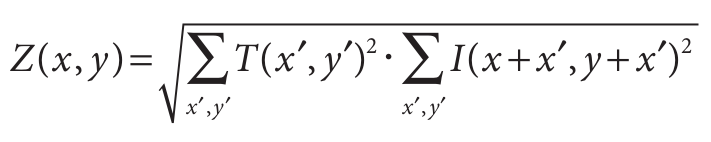
\includegraphics[scale=0.3]{/home/nicgen/Scrivania/thesis/Figures/z.png}
\caption[Coefficiente normalizzato]{Coefficiente normalizzato}
\label{pic-a}
\end{figure}

Si definisce infine il metodo CV\_TM\_CCORR\_NORMED come:

\begin{figure}[H]\centering  
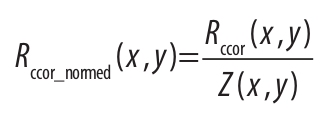
\includegraphics[scale=0.38]{/home/nicgen/Scrivania/thesis/Figures/rccor.png}
\caption[Correlation matching method formula (normed)]{Correlation matching method formula (normed)}
\label{pic-a}
\end{figure}

Vi sono anche metodi basati sulla differenza di quadrati ma si è preferito utilizzare dei metodi piu sofisticati in quanto assicurano risultati migliori (tenendo conto della bassa qualità dei fotogrammi in entrata dovuta a fotocamere con sensori ridotti).





\newpage
\subsection{Stima della posa}

Tale funzionalità nasce dalla necessità di gestire il fotogramma in ingresso in base all'inclinazione ed orientamento del volto dell'utente rispetto alla camera. Come già espresso in precedenza, infatti, la meccanica OpenCV per Android si limita a riconoscere solamente volti quasi perfettamente frontali alla camera. Lo studio effettuato è stato mirato a gestire i casi in cui il volto fosse inclinato. Infatti, ottenuti tali informazioni sulla posa, sarebbe stato possibile capire l'inclinazione del volto e di conseguenza ruotare il fotogramma (a tempo di esecuzione) in ingresso per facilitare il riconoscimento da parte del motore. Dal momento che tale funzionalità doveva essere disponibile su dispositivi mobili, sono state effettuate considerazioni prestazionali (test prototipali avevano evidenziato una notevole diminuzione di performance di sistema aggiungendo al rilevamento facciale principale il riconoscimento di una singola parte). 

Pertanto sono state considerate solamente le seguenti parti:

\begin{itemize}
\item Occhio Sinistro viene ad esso associato la cascata cascade\_eye\_sx (Haar)
\item Occhio Destro viene ad esso associato la cascata cascade\_eye\_dx (Haar)
\item Bocca viene ad esso associato la cascata cascade\_mouth (Haar)
\end{itemize}

Per valutare la fattibilità è stata creata una semplice funzione che imprimesse direttamente sul fotogramma un triangolo i cui vertici corrispondono alle parti sopracitate.

\begin{figure}[H]\centering  
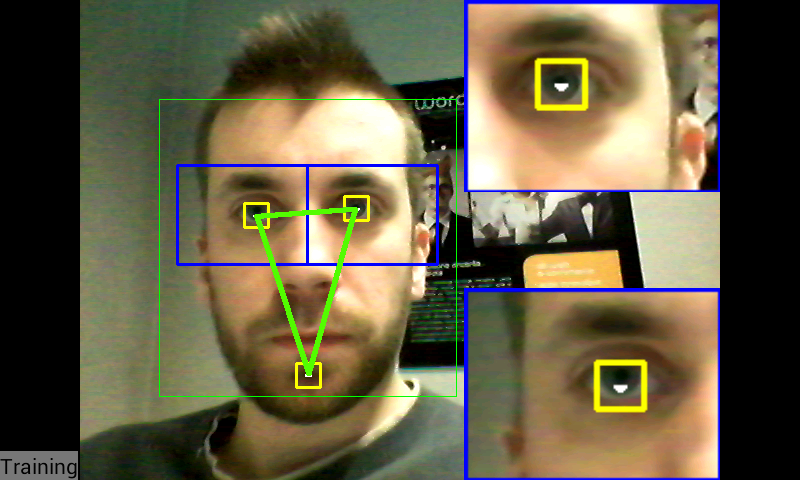
\includegraphics[scale=0.38]{/home/nicgen/Scrivania/thesis/Figures/face1_triangle.png}
\caption[Risultato visivo della triangolazione]{Risultato visivo della triangolazione}
\label{pic-a}
\end{figure}

E' stata successivamente creata una funzione che, in base alle fattezze del triangolo, potesse ricavare l'inclinazione del volto. Ottenuti infatti i punti degli occhi, ottengo una retta ed utilizzando della semplice trigonometria trovo l'angolo cercato. A confermare tale cambiamento di rotazione (che viene salvata in un buffer di posizioni) deve essere la posizione della bocca rispetto all'interno del fotogramma.

Dai test effettuati su un prototipo usa e getta sono state evidenziate le seguenti problematiche:

\begin{itemize}
\item La generazione di un template (che avviene ciclicamente ogni secondo per alcuni frame) non garantisce che la posizione della parte trovata coincida con la posizione reale. Se ad esempio la generazione del template avviene un solo occhio è eccessivamente aperto, ci si potrebbe ritrovare in fase di mantenimento ad avere una posizione scorretta fino al successivo evento di generazione template. Quindi, nonostante il volto sia perfettamente frontale, può venire inoltrato al motore OpenCV una richiesta di rotazione della matrice immagine che si traduce in instabilità generale del rilevamento.
\item Le condizioni d'utilizzo (in particolare la luminosità dell'ambiente) possono influire sul risultato: è necessaria quindi un metodo che mantenga la fedeltà del volto individuato per ogni fotogramma. Tale metodo memorizzerà la posizione del rettangolo contenente il volto, la posizione dei rettangoli contenenti occhi e bocca, e le posizioni puntuali di queste ultime parti.
\item Il costo computazionale della creazione dei templates in questo caso è molto elevato e il framerate massimo raggiunto è di 10 fotogrammi al secondo su uno smartphone di fascia alta \textit{(Galaxy S4)}. A questo si aggiunge il costo di rotazione della matrice immagine.
\item Tale approccio può funzionare solo se l'utilizzatore dell'applicazione è unico (non viene gestito il caso in cui la camera trovi più di un volto)
\end{itemize}			

OpenCV fornisce altri strumenti molto potenti come ad esempio \textit{CamShift} ma non è stata possibile un'implementazione a causa dei vincoli sulla tabella di lavoro. Pertanto non è stato possibile eseguire uno studio di fattibilità adeguato per la risoluzione di tale problematica. 


\newpage
\subsection{Calibrazione dinamica}

 
%\chapter{Verifica e Validazione} % Main chapter title

\label{Capitolo5} % For referencing the chapter elsewhere, use \ref{Chapter1} 

\lhead{Capitolo 5. \emph{Verifica e Validazione}} % This is for the header on each page - perhaps a shortened title

\section{Analisi Statica}
Al fine di portare avanti il processo di verifica con metodo è stato necessario renderlo
quantificabile. Perciò si sono definite delle metriche sul codice sorgente. Esse sono
di seguito definite e il loro significato viene descritto e spiegato. Per ogni metrica si
sono definiti un range di accettazione e un range ottimale.

\subsection{Complessità ciclomatica}

Tale metrica indica il numero di cammini linearmente indipendenti percorribili durante
l'esecuzione di un singolo metodo. Tale metrica è molto importante in quanto ha
implicazioni dirette sulle attività di testing: infatti essa rappresenta un upper bound
per il numero di routine di test necessarie per raggiungere un completo branch coverage.

\textbf{Range dichiarato:}
\begin{itemize}
\item Accettazione $\leq 15$
\item Ottimale $\leq 10$
\end{itemize}

\subsection{LOC}

Tale metrica (Lines of Code, linee di codice) indica il numero di linee di codice. Nel conteggio vengono escluse le righe contenenti dichiarazioni di namespaces, tipi, campi, metodi oltre che i metodi astratti e i tipi enumeration.
Solo il codice effettivamente eseguito è considerato nel conteggio delle righe.
La metrica LOC non è sempre legata alla produttività del programmatore, ma torna
utile sia nel calcolo della percentuale di statement coverage e nella valutazione del
software.
Essa è indice di manutenibilià (è più semplice manutenere metodi brevi) e quindi
qualità del codice.

\textbf{Range per metodo:}
\begin{itemize}
\item Accettazione $\leq 45$
\item Ottimale $\leq 15$
\end{itemize}

\subsection{Numero di campi utilizzati per classe}

Indica il numero di membri di classe (campi dati) di una particolare classe. E'
importante in quanto è indice delle responsabilità andate ad una classe, se viene
superato può indicare che la classe ne raggruppa troppe altre e andrebbe ulteriormente
separata in classi distinte.

\textbf{Range dichiarato:}
\begin{itemize}
\item Accettazione $\leq 16$
\item Ottimale $\leq 8$
\end{itemize}

\subsection{Numero di metodi utilizzati per classe}

Indica il numero di metodi di una particolare classe. Similmente al numero di campi
per classe è importante in quanto è indice delle responsabilità andate ad una classe, se
viene superato può indicare che la classe ha troppe funzionalità e andrebbe separata.

\textbf{Range dichiarato:}
\begin{itemize}
\item Accettazione $\leq 16$
\item Ottimale $\leq 8$
\end{itemize}

\subsection{LCOM e LCOM HS}

Si vuole definire una metrica a partire da questa definizione: se una classe ha una sola responsabilità si
dice che essa è coesa. In generale una classe risulterà coesa se i suoi metodi sono
strettamente legati fra loro. Quando metodi distinti non usano attributi o metodi
comuni significa che essi non condividono nulla e che quindi potrebbero venir separati.
La metrica di LCOM misura quindi quanto poco una classe è coesa. Alcune formule per il
calcolo di LCOM sono le seguenti:

\begin{center}
\textbf{LCOM} =  $1-(\sum(MF)/M \ast F) $  \\
\textbf{LCOM HS} = $(M-(\sum(MF)/F))\ast(M-1)$
\end{center}

Dove:
\begin{itemize}
\item M è il numero di metodi nella classe. Si considerano sia i metodi statici sia quelli di istanza, ed include inoltre i costruttori,getters e setters ed eventuali metodi del tipo add/remove
\item F è il numero di campi dati d'istanza all'interno della classe 
\item MF è il numero di metodi della classe che accedono un particolare campo dati di tipo classe
\item $\sum(MF)$ è la somma degli MF tra tutti i campi d'istanza della classe
\end{itemize}

L'idea alla base di tali formule è che una classe perfettamente coesa utilizza tutti i
suoi campi dati di tipo classe all'interno di ogni suo metodo il che comporta :

\begin{center}
 $(\sum(MF) = M \ast F) \Leftrightarrow LCOM = 0 $
\end{center}

La differenza tra LCOM e la sua versione HS (Hendersons-Sellers) è che la prima
ritorna dei valori nel range [0-1] mentre la seconda nel range [1-2]. La versione HS è
considerata più efficace per la rilevazione dei tipi scarsamente coesi.
Tale metrica è interessante, ma va trattata con cautela (basti pensare una classe
che ha n campi dati, n getters e n setters, essa risulterà scarsamente coesa, il che
non rispecchia la realtà). Infatti essa non va valutata singolarmente, ma deve essere
inserita in un contesto di valutazione che comprende altre variabili, soprattutto il
numero di campi e il numero di metodi. 

\textbf{Range dichiarato:}
\begin{itemize}
\item Accettazione $\leq 0.8$
\item Ottimale = 0
\end{itemize}

\newpage
\section{Analisi Dinamica}

Nello sviluppo dell'applicazione si sono progettati dei test che precedessero l'implementazione di ogni componente e di ogni classe. I test di integrazione hanno definito come i vari
componenti avrebbero dovuto relazionarsi tra di loro, e per ogni componente sono stati definiti adeguati test di unità che andassero a verificare il corretto funzionamento delle classi interne. Ogni unità e stata testata in
relazione al ruolo che essa avrebbe avuto all'interno del sistema in base al suo "peso".
I test d'unità verificano in gran parte l'integrità degli input inseriti dall'utente e di come questi variano durante l'utilizzo dell'applicativo.

Per l'analisi delle chiamate ai metodi forniti dalle librerie esterne (OpenCV e Facebook SDK) si è cercato di
verificare la correttezza nei limiti di risorse e tempo disponibili. Infatti alcune funzioni fornite da tali librerie sono ad alto livello e comprendono un grafo di chiamate molto esteso
(in particolare chiamate a metodi di OpenCV, come il rilevamento facciale, e a Facebook per quanto riguarda il login e il mantenimento della sessione attiva), e non è stato possibile progettare test in quanto tali operazioni sono
particolarmente complesse e avrebbero richiesto una profonda comprensione della meccanica di tali librerie.

Il tool utilizzato per eseguire i test è stato Android JUnit che fornisce delle classi previste di metodi adibiti alla creazione dei cosiddetti oggetti mock (oggetti simili a quelli reali ma che hanno l'obiettivo di simulare l'oggetto reale in maniera controllata) e metodi che possano aiutare ad aiutare il ciclo di vita di un componente.

\section{Test di Validazione}

Vengono riportati in questa sezione i test che descrivono la strategia utilizzata per la
validazione del prodotto. Si è cercato di tenere un rapporto di 1:1 tra i
requisiti funzionali e i test di validazione che verificavano quella specifica funzionalità.
Per ogni test viene riportato il suo codice gerarchico identificativo. Se tale test risulta sufficientemente grande, esso viene scomposto in sotto-test aventi come indice gerarchico l'indice del padre.

\begin{itemize}
\item \textbf{T1} Il test è atto a verificare il buon funzionamento dell'attività di riconoscimento facciale e delle rispettive parti
\begin{itemize}
\item \textbf{T1.1} Il test verifica il corretto caricamento delle librerie e le adatta in base all'hardware caratterizzante dispositivo
\item \textbf{T1.2} Il test verifica la possibilità di eseguire la calibrazione con le
impostazioni selezionate
\begin{itemize}
\item \textbf{T1.2.1} Il test verifica la possibilità di cambiare camera a run-time
\item \textbf{T1.2.2} Il test verifica la possibilità di cambiare il tipo di elaboratore della camera
\item \textbf{T1.2.3} Il test verifica la possibilità di cambiare la risoluzione del frame in ingresso
\item \textbf{T1.2.4} Il test verifica la possibilità di cambiare il range operativo di campionamento
\item \textbf{T1.2.5} Il test verifica la possibilità di cambiare i parametri operativi di campionamento
\item \textbf{T1.2.6} Il test verifica il corretto funzionamento di modifica delle parti da ricercare a run-time
\item \textbf{T1.2.7} Il test verifica la possibilità di abilitare o disabilitare la modalità alto contrasto e/o monocromatica
\end{itemize}


\item \textbf{T1.4} Il test verifica la possibilità di cambiare lo Sprite corrente
\begin{itemize}
\item \textbf{T1.4.1} Il test deve verificare il corretto caricamento degli Sprites
\item \textbf{T1.4.2} Il test deve verificare la corretta renderizzazione della ListView
\item \textbf{T1.4.3} Il test verifica verifica il corretto utilizzo dello Sprite assegnato
\end{itemize}
\end{itemize}
\item \textbf{T2.1} Il test verifica il corretto caricamento di un'immagine dallo smartphone
\item \textbf{T3} Il test verifica la possibilità di condividere la foto
\begin{itemize}
\item \textbf{T3.1} Il test verifica la possibilità di ridimensionare la foto scattata
\item \textbf{T3.2} Il test verifica la possibilità di condividere la foto inoltrandola verso applicazioni di messaggistica preinstallate nello smartphone
\begin{itemize}
\item \textbf{T3.2.1} Il test verifica il caricamento della lista di applicazioni attraverso le quali è possibile condividere il contenuto
\item \textbf{T3.2.2} Il test verifica l'esito della condivisione
\end{itemize}
\item \textbf{T3.3} Il test verifica la possibilità di eseguire la connessione verso la piattaforma Facebook
\begin{itemize}
\item \textbf{T3.3.1} Il test verifica la possibilità di eseguire il Login sulla piattaforma Facebook
\item \textbf{T3.3.2} Il test verifica il mantenimento della sessione successivo alla chiusura dell'applicazione
\item \textbf{T3.3.3} Il test verifica l'integrità dei dati allegati alla foto, inseriti dall'utente
\item \textbf{T3.3.4} Il test verifica l'esito della condivisione
\end{itemize}
\end{itemize}
\end{itemize}

 
%\chapter{Esiti Attività} % Main chapter title

\label{Capitolo6} % For referencing the chapter elsewhere, use \ref{Chapter1} 

\lhead{Capitolo 6. \emph{Esiti Attività}} % This is for the header on each page - perhaps a shortened title



\section{Esiti Analisi Statica}

Di seguito vengono riportati i risultati dell'analisi statica sul codice sorgente effettuata
con lo strumento JTest. Vengono riportati per ogni
classe:
\begin{itemize}


\item Classe: il nome della classe preceduto dall'indicazione del componente padre
\item CC: per la metrica di complessità ciclomatica viene riportato il valore ottenuto
dalla media aritmetica dei vari metodi di classe 
\item LOC: per la metrica di linee di codice viene riportato il valore intero ottenuto dalla
media aritmetica dei vari metodi di classe (per evitare di riportare i singoli
metodi)
\item LCOM HS:
il valore ottenuto dal calcolo della metrica LCOM HS che indica la
coesione dei metodi di una classe.

\end{itemize}

Il numero di campi dati e di metodi utilizzati per classe è una diretta fonte dei risultati ottenuti.


\begin{center}
    \begin{longtable}{ | p{6cm} | p{1.5cm} | p{1.5cm} | p{1.8cm} |}
    \hline
    Classe & CC & LOC & LCOM HS \\ \hline
    Activity::SplashScreenActivity& 1.2 & 5 & 0.15\\ \hline 
    Activity::FaceDetectionActivity& 3.33 & 15& 1.37\\ \hline 
    Activity::StaticFaceDetectionActivity& 1.81 & 12 & 0.8\\ \hline 
    Activity::PhotoActivity& 2.34 & 8 & 0.73\\ \hline 
    Activity::TutorialActivity& 2.55 & 4  & 0.42\\ \hline 
    Service::BootStartUpReceiver & 1 & 3 & 0.25\\ \hline 
    Service::BackgroundService & 1.33 & 5 & 0.25\\ \hline 
    Model::Data& 1.66 &  6  & 1.84\\ \hline 
    Model::Templates& 3.11 & 11  & 0\\ \hline 
    Model::Sprite& 1.82 & 5  & 0.51\\ \hline 
    Core::Camera& 1.2 & 12 & 0\\ \hline 
    Social::LoginSession& 2.73 & 5 & 0.15\\ \hline 
    Social::Share& 1.55 & 7 & 0\\ \hline 
    Utility::MatUtils& 1.27 & 5 & 0\\ \hline 
	Utility::Generics& 3.83 & 13 & 0\\ \hline 
	Adapter::CustomAdapter& 1.17 & 6 & 0.15\\ \hline     
    


    \end{longtable}
\end{center}

Complice la ridotta esperienza, durante lo sviluppo è stato necessario rivisitare ed affinare alcuni metodi per rientrare nel range di accettazione per la complessità ciclomatica scomponendo il problema in sotto-problemi di minore dimensioni e quindi più facilmente verificabili. A seguito di alcune controlli del codice tutti i limiti imposti sono stati rispettati.
Nella tabella a seguire sono presenti valori di \textit{LCOM HS} $=$ 0. Ciò possibile in quanto nella classe non sono presenti campi dati. Sono però presenti anche valori \textit{LCOM HS} > 1.0, che potrebbero indicare un campanello d'allarme. Nonostante sia difficile evitare tale problema, una migliore progettazione avrebbe potuto produrre valori di coesione migliori.


\section{Esiti Test di Validazione}

\begin{center}
    \begin{longtable}{ | p{2cm} | p{6cm} | p{2cm} | p{2cm} |}
    \hline
    Codice & Descrizione & Requisito & Esito \\ \hline
        & Verificato dal buon esito dei figli &RFO1 & \textcolor{green}{Positivo}\\ \hline 
    T1.1& Verificare il corretto funzionamento dell'attività e il caricamento dinamico dei parametri d'utilizzo in base al dispositivo utilizzato &RFO1.1 & \textcolor{green}{Positivo}\\ \hline 
    T1.2& Verificato dal buon esito dei figli  &RFO1.2 & \textcolor{green}{Positivo}\\ \hline 
    T1.2.1& Verificare la possibilità di cambiare camera a tempo d'esecuzione &RFO1.2.1 & \textcolor{green}{Positivo}\\ \hline 
    T1.2.2& Verifica la possibilità di cambiare l'elaborazione della camera (Nativa o Java) &RFO1.2.2 & \textcolor{green}{Positivo}\\ \hline 
   T1.2.3 &Verifica la possibilità di cambiare la risoluzione del frame in ingresso&RFO1.2.3 & \textcolor{green}{Positivo}\\ \hline 
    T1.2.4& Il test verifica la possibilità di cambiare il range operativo di campionamento &RFO1.2.4 & \textcolor{green}{Positivo}\\ \hline 
    T1.2.5&Il test verifica la possibilità di cambiare i parametri operativi di campiona-
mento &RFO1.2.5 & \textcolor{green}{Positivo}\\ \hline 
    T1.2.6&Il test verifica il corretto funzionamento di modifica delle parti da ricercare a
run-time &RFO1.2.6 & \textcolor{green}{Positivo}\\ \hline 
    T1.2.7&Il test verifica la possibilità di abilitare o disabilitare la modalità alto contrasto
e/o monocromatica &RFO1.2.7 & \textcolor{green}{Positivo}\\ \hline 
    T1.4& Verificato dal buon esito dei figli &RFD1.4 & \textcolor{green}{Positivo}\\ \hline 
    T1.4.1&Il test deve verificare il corretto caricamento degli Sprites &RFO1.4.1 & \textcolor{green}{Positivo}\\ \hline 
    T1.4.2&Il test deve verificare la corretta renderizzazione della ListView &RFO1.4.2 & \textcolor{green}{Positivo}\\ \hline 
    T1.4.3&Il test verifica verifica il corretto utilizzo dello Sprite assegnato &RFO1.4.3& \textcolor{green}{Positivo}\\ \hline 
    T2.1&Il test verifica il corretto caricamento di un'immagine dallo smartphone &RFO2.1  & \textcolor{green}{Positivo}\\ \hline 
    T3& Verificato dal buon esito dei figli &RFO3 & \textcolor{green}{Positivo}\\ \hline 
    T3.1& Il test verifica la possibilità di ridimensionare la foto scattata &RFD3.1 & \textcolor{green}{Positivo}\\ \hline 
    T3.2& Verificato dal buon esito dei figli &RFD3.2  & \textcolor{green}{Positivo}\\ \hline 
    T3.2.1&Il test verifica il caricamento della lista di applicazioni attraverso le quali
`e possibile condividere il contenuto &RFD3.2.1  & \textcolor{green}{Positivo}\\ \hline 
    T3.2.2&Il test verifica l'esito della condivisione&RFD3.2.2  & \textcolor{green}{Positivo}\\ \hline 
    T3.3& Verificato dal buon esito dei figli &RFD3.3  & \textcolor{green}{Positivo}\\ \hline 
    T3.3.1& Il test verifica la possibilità di eseguire il Login sulla piattaforma Facebook &RFD3.3.1  & \textcolor{green}{Positivo}\\ \hline 
    T3.3.2&Il test verifica il mantenimento della sessione successivo alla chiusura
dell'applicazione &RFD3.3.1  & \textcolor{green}{Positivo}\\ \hline 
    T3.3.3& Il test verifica l'integrità dei dati allegati alla foto, inseriti dall'utente &RFD3.3.2  & \textcolor{green}{Positivo}\\ \hline 
    T3.3.4& Il test verifica il caricamento e l'esito della condivisione&RFD3.3.3  & \textcolor{green}{Positivo}\\ \hline 
    \end{longtable}
\end{center}


\section{Analisi Prestazionale}

Al fine di verificare le prestazioni ottenute in media dall'applicativo, l'azienda ha fornito 4 dispositivi che rappresentano all'anno della stesura di questo documento (2014) le possibili fasce di mercato.

I dispositivi forniti sono:

\begin{itemize}
\item \textbf{Fascia Alta - \textit{Galaxy S4}} 
	\begin{itemize}
		\item CPU quad core 1.6GHz Cortex A15 
		\item RAM 2 GB 
		\item Fotocamera : posteriore: 13 MP , anteriore 2.1 MP
		\item Android 4.2.2 Jelly Bean 
	\end{itemize}
\item \textbf{Fascia Media - \textit{Galaxy S3 Mini}}
	\begin{itemize}
		\item CPU 1 GHz dual core ARM Cortex A9
		\item RAM 1 GB 
		\item Fotocamera : posteriore: 5 MP , anteriore 1.3 MP
		\item Android 4.1.1 Jelly Bean 
	\end{itemize}
\item \textbf{Fascia Bassa - \textit{Galaxy Fame}}
	\begin{itemize}
		\item CPU 0.85 GHz single core ARM Cortex A9
		\item RAM 512 MB
		\item Fotocamera : posteriore: 3 MP , anteriore 1.3 MP
		\item Android 2.3.0 Gingerbread
	\end{itemize}
\end{itemize}

Dal momento che le prestazioni possono dipendere dalla qualità della luce e dalla distanza dell utente dal dispositivo, si è preferito testare l'applicazione utilizzando video come input. Le variabili tenute in considerazione sono risoluzione, numero di volti, numero di falsi positivi, numero di fotogrammi medi per secondo al termine di ogni video. I video sono sono volutamente caratterizzati da camere mobili, e da scene in cui non sono presenti persone al fine di verificare la presenza di falsi positivi.

I video utilizzati sono reperibili direttamente dal web ai link:

\begin{itemize}
\item[•] \href{http://www.youtube.com/watch?v=XFTbN10f_Fg}{Video 1 : Matrix - The red Woman}
\item[•] \href{http://www.youtube.com/watch?v=yWPyRSURYFQ}{Video 2 : Blade Runner - She's a Replicant}
\item[•] \href{http://www.youtube.com/watch?v=s3rv0BdxWfM}{Video 3 : The Heat - The Sun Rises and Sets With Her }
\end{itemize}

Risoluzioni utilizzate:

\begin{itemize}
\item[•] $1280\ast720$ 
\item[•] $640\ast480$ 
\item[•] $320\ast240$ 
\end{itemize}

I test sono stati effettuati con i seguenti parametri precedentemente definiti in sezione:
\begin{itemize}
\item \textit{FaceDetectionActivity::minNeighbors} = 3 (sono necessari almeno 3 hit per frame per confermare positivamente il volto)
\item \textit{FaceDetectionActivity::minSize} = -1  
\item \textit{FaceDetectionActivity::maxSize} = -1
\item \textit{FaceDetectionActivity::scaleFactor} = 1.1 
\end{itemize}

In questo modo ci si assicura che il costo computazionale per ogni frame sia massimo (il metodo di rilevamento facciale terminerà solo dopo aver valutato l'immagine nella sua interezza). 
Dato che per ogni singolo frame vi possono essere più hits corrispondenti allo stesso volto, è stata creata una semplice funzione ad hoc che permetta di contare un solo volto per set coincidenti di hits. Inoltre tali video sono stati velocizzati aumentando il framerate (24$\longmapsto$ 72 fotogrammi per secondo) per evitare qualsiasi problema di Input bound.


\begin{figure}[h]\centering  
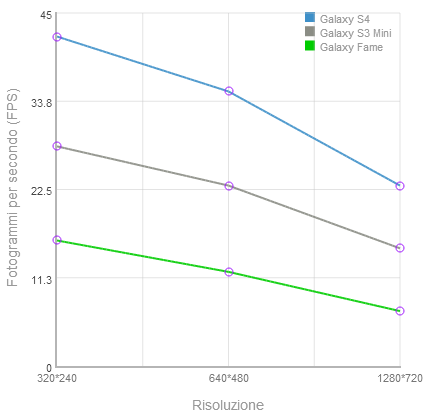
\includegraphics[scale=0.6]{/home/nicgen/Scrivania/thesis/Figures/fps.png}
\caption[Grafico prestazionale riassuntivo]{Graifco prestazionale riassuntivo}
\label{pic-a}
\end{figure}

Come previsto, al variare dei dispositivi non vi è alcuna differenza nei risultati (quantità di volti rilevati + $\varepsilon$(falsi positivi rilevati)) se non al variare del parametro \textit{FaceDetectionActivity::MinNeighbors}. Infatti,prendendo come risoluzione di riferimento $640 \ast 480$, sono stati ottenuti i seguenti risultati
\\
GRAFICO A RES FISSA CON NUM FALSI POSITIVI E NEGATIVI AL VARIARE DELLA RETENTION 
\\
I risultati sono però stati totalmente differenti nell'utilizzo reale utilizzando la fotocamera posteriore come input al posto dei video (che garantivano un framerate costante di 72 fotogrammi per secondo). 
\\
GRAFICO LUMINOSITA NORMALE

GRAFICO LUMINOSITA BASSA
\\
Infine si può notare come vi siano grosse discrepanze di prestazioni al variare della fotocamera d'input (Anteriore o Posteriore). Questo è dovuto al fatto che generalmente la fotocamera posteriore è di qualità maggiore (sensore di dimensioni maggiori, diaframma più aperto ed ISO che può raggiungere valori più elevati)
\\
GRAFICO FRONTALE VS POSTERIORE

\subsection{Considerazioni}

A seguito dei test effettuati l'idea è che i dispositivi correntemente presenti sul mercato abbiamo una potenza computazionale più che sufficiente per eseguire tali task con prestazioni discrete e garantiscano un'esperienza d'utilizzo adeguata. Il maggior problema riscontrato è sicuramente la qualità della fotocamera che può condizionare drasticamente le performance se posta in condizione d'utilizzo non ottimale. Il software preinstallato sullo smartphone infatti, in condizioni di bassa luminosità, tende ad alzare il valore ISO (sensibilità del sensore) ed ad utilizzare un diaframma il più aperto possibile. La necessità di miniaturizzare l'hardware fotografico ha però come conseguenza quella di non poter avere sensori e lenti di dimensioni adeguate. Questo si traduce in bassa qualità, e pertanto per ogni singolo frame di un video sarà necessario un tempo di esposizione molto elevato. Lo stream di fotogrammi risulterà quindi caratterizzato da un framerate molto basso, ponendo il processore in attesa attiva del fotogramma da processare. 

 
%% Chapter 1

\chapter{Valutazione retrospettiva} % Main chapter title

\label{Chapter4} % For referencing the chapter elsewhere, use \ref{Chapter1} 

\lhead{Capitolo 4. \emph{Valutazione Retrospettiva}} % This is for the header on each page - perhaps a shortened title

%----------------------------------------------------------------------------------------

\section{Copertura dei Requisiti}

Vengono riportate le tabelle con gli esiti dell'attività di sviluppo. Per ogni
requisito viene riportato l'esito dello stesso dopo lo sviluppo e l'implementazione del
software. L'esito è stato diviso nelle seguenti categorie:
\begin{itemize}
\item \textbf{Soddisfatto:} Indica che il requisito è stato implementato con successo e quindi
soddisfatto. Colore associato \textcolor{green}{verde}
\item \textbf{Non soddisfatto:} Indica che il requisito non è stato implementato con successo.
Colore associato \textcolor{red}{rosso}
\item \textbf{Incompleto:} Indica che il requisito è stato implementato solo in alcune sue
parti o che il risultato non è stato raggiunto in modo soddisfacente. Colore associato \textcolor{gray}{grigio}
\end{itemize}

\begin{center}
    \begin{longtable}{ | p{2cm} | p{7cm} | p{2cm} |}
    \hline
    Requisiti & Descrizione & Esito \\ \hline
    RFO1 &  L'applicazione deve permettere il rilevamento facciale in tempo reale su dispositivi mobili Android & \textcolor{green}{Soddisfatto}  \\ \hline 
    RFO1.1 &  L'applicazione deve permettere di avviare il training OpenCV  & \textcolor{green}{Soddisfatto} \\ \hline
    RFO1.2 &  L'applicazione deve permettere di calibrare la camera corrente  & \textcolor{green}{Soddisfatto}  \\ \hline 
    RFO1.2.1 &  L'applicazione deve permettere all'utente di selezionare la camera desiderata & \textcolor{green}{Soddisfatto} \\ \hline
    RFO1.2.2 &  L'applicazione deve permettere all'utente di modificare il tipo di elaborazione della camera & \textcolor{green}{Soddisfatto} \\ \hline
    RFO1.2.3 &  L'applicazione deve permettere all'utente di modificare la risoluzione del frame in ingresso & \textcolor{green}{Soddisfatto}  \\ \hline
    RFO1.2.4 &  L'applicazione deve permettere all'utente di modificare la profondità di campionamento (distanza minima e massima su cui effettuare lo scan) & \textcolor{green}{Soddisfatto}  \\ \hline
    RFO1.2.5 &  L'applicazione deve permettere all'utente di modificare il numero minimo di campionamenti sotto il quale il volto non viene riconosciuto come valido  & \textcolor{green}{Soddisfatto}  \\ \hline
    RFO1.2.6 &  L'applicazione deve permettere all'utente di abilitare di abilitare/disabilitare la ricerca delle features in tempo reale  & \textcolor{green}{Soddisfatto}  \\ \hline
    RFO1.2.7 &  L'applicazione deve permettere all'utente di abilitare/disabilitare la modalità contrasto e/o monocromatica  & \textcolor{green}{Soddisfatto}  \\ \hline
    RFD1.3 &  L'applicazione deve permettere di cogliere l'orientamento dell'eventuale volto individuato & \textcolor{gray}{Incompleto} \\ \hline    
    RFD1.4 &  L'applicazione deve permettere di scegliere lo Sprite da utilizzare & \textcolor{green}{Soddisfatto} \\ \hline    
    RFO1.4.1 &  L'applicazione deve caricare una lista di Sprites, che saranno successivamente selezionabili dall'utente & \textcolor{green}{Soddisfatto}  \\ \hline
    RFO1.4.2 &  L'applicazione deve permettere all'utente di selezionare uno o più Sprites desiderati da una ListView presente all'interno dell'interfaccia grafica  & \textcolor{green}{Soddisfatto}  \\ \hline
    RFO1.4.3 &  L'applicazione deve poter renderizzare gli Sprites precedentemente selezionati & \textcolor{green}{Soddisfatto} \\ \hline    
    RFO2 &  L'applicazione deve permettere di rilevare volti a partire da un immagine statica su dispositivi mobili Android & \textcolor{green}{Soddisfatto}  \\ \hline
    RFO2.1 &  L'applicazione deve permettere all'utente di caricare una foto dal proprio smartphone & \textcolor{green}{Soddisfatto}  \\ \hline
    RFO2.2 &  L'applicazione deve permettere di avviare il rilevamento facciale & \textcolor{green}{Soddisfatto} \\ \hline
    RFD2.3 &   L'applicazione deve permettere di scegliere uno o più Sprites da utilizzare  & \textcolor{green}{Soddisfatto}  \\ \hline 
    RFO3 &  L'applicazione deve permettere la condivisione di contenuti multimediali & \textcolor{green}{Soddisfatto} \\ \hline
    RFD3.1 &  L'applicazione deve permettere di ridimensionare la foto scattata in base a formati predefiniti & \textcolor{green}{Soddisfatto} \\ \hline
    RFD3.2 &  L'applicazione deve permettere di condividere la foto ottenuta verso applicazioni di messaggistica interne  & \textcolor{green}{Soddisfatto} \\ \hline
    RFD3.2.1 &  L'applicazione deve fornire l'utente di un bottone attraverso il quale può esprimere il suo intento di condividere il contenuto  & \textcolor{green}{Soddisfatto} \\ \hline
    RFD3.2.2 &  L'applicazione deve rispondere fornendo graficamente una risposta contenente i servizi di inoltro disponibili  & \textcolor{green}{Soddisfatto} \\ \hline
    RFD3.2.3 &  L'applicazione deve condividere il contenuto multimediale attraverso il servizio selezionato  & \textcolor{green}{Soddisfatto} \\ \hline    
    RFD3.3 &  L'applicazione deve permettere il login facebook e condividere la foto su quest ultimo  & \textcolor{green}{Soddisfatto} \\ \hline
    RFD3.3.1 &  L'applicazione deve permettere l'inoltro di una richiesta di accesso verso i server Facebook & \textcolor{green}{Soddisfatto} \\ \hline
    RFD3.3.2 &  L'applicazione deve permettere l'inserimento di un testo da allegare alla foto & \textcolor{green}{Soddisfatto} \\ \hline
    RFD3.3.3 &  L'applicazione deve permettere il caricamento della foto sulla piattaforma Facebook & \textcolor{green}{Soddisfatto} \\ \hline
    RFD4 &  L'applicazione deve mantenere un framerate minimo di 15 fotogrammi al secondo & \textcolor{red}{Non Soddisfatto} \\ \hline
    \end{longtable}
\end{center}


%----------------------------------------------------------------------------------------
\newpage
\section{Prodotto finale}



\section{Conoscenze acquisite}

Durante l'esperienza di stage ho approfondito le mie capacità in ognuna delle fasi principali
dello sviluppo software. Ho avuto modo di sviluppare competenze in diverse tecnologie e nel loro uso. Le più rilevanti dal mio punto di vista sono le seguenti:

\begin{itemize}
\item \textbf{Java} Le precedenti conoscenze teoriche apprese durante il corso di Programmazione Concorrente e Distribuita sono state applicate in maniera concreta di fronte a problemi reali. 
\item \textbf{Android Studio} Le conoscenze riguardo a questo ambiente prima dell'inizio dello stage erano pressochè nulle in quanto non mi ero mai trovato ad affrontare
questo argomento. Ho avuto modo di conoscere ed ad utilizzare parte dell'enorme mole di strumenti offerti allo sviluppatore, in particolar modo quelli dediti al debug (DDMS), all'analisi della memoria e alla suite di test.
\item \textbf{Facebook} Le conoscenze riguardo a questo ambiente prima dell'inizio dello stage erano pressochè nulle. Grazie ai numerosi tutorial ufficiali presenti in rete è stato possibile realizzare facilmente i requisiti definiti.
\item \textbf{OpenCV} Lo studio di tale libreria mi ha permesso di conoscere, nei limiti del tempo concesso per lo stage, questo variegato strumento di analisi ed elaborazione delle immagini. In particolar modo è stato molto interessante lo studio di come gli oggetti vengono campionati per poi essere utilizzati all'interno di un classificatore. Inoltre, a fini prestazionali, è stata significativa l'analisi effettuata per variare i parametri di rilevamento in base all'hardware presente sul dispositivo. 
\end{itemize}

%----------------------------------------------------------------------------------------



%----------------------------------------------------------------------------------------

\section{Conoscenze possedute e relazione con la preparazione accademica}

Durante lo svolgimento dello stage si sono potute applicare le conoscenze già
acquisite per la gestione di progetto e per il miglior sviluppo possibile dell'applicazione,
potendo provare sul campo l'importanza dell'analisi dei requisiti e della
validazione, i benefici di una attenta progettazione dell'architettura e
di una strategia formale ed estensiva di test del prodotto.
Credo che la preparazione accademica precedente all'attività di stage
sia stata adeguata perché potessi affrontare al meglio il progetto, non tanto
nelle conoscenze fornite quanto piuttosto nel metodo insegnato durante tutti i
corsi del percorso di laurea triennale. Inoltre il supporto del tutor aziendale Marcus Oblack mi ha dato la motivazione e la curiosità di informarmi sulle tecnologie necessarie per condurre in maniera efficace la creazione di questo progetto.

Per concludere penso che questo percorso sia stato impegnativo, vivo e stimolante. Mi ha
permesso di mettere in pratica le conoscenze e le capacità acquisite durante la mia vita ed il mio il percorso di studi. Mi ritengo quindi pienamente soddisfatto del suo esito finale.

 

%----------------------------------------------------------------------------------------
%	THESIS CONTENT - APPENDICES
%----------------------------------------------------------------------------------------

\addtocontents{toc}{\vspace{2em}} % Add a gap in the Contents, for aesthetics

\appendix % Cue to tell LaTeX that the following 'chapters' are Appendices

% Include the appendices of the thesis as separate files from the Appendices folder
% Uncomment the lines as you write the Appendices

% Appendix A

\newpage
\chapter{Glossario} % Main appendix title
\renewcommand{\chaptername}{MyChapter}
\label{AppendixA} % For referencing this appendix elsewhere, use \ref{AppendixA}

\lhead{\emph{Glossario}} % This is for the header on each page - perhaps a shortened title

\textbf{Ant:} libreria Java il cui compito è quello di guidare il processo di build di applicazioni Java. Fornisce numerose funzionalità in grado di di compilare, assemblare, testare ed avviare le applicazioni.


\textbf{Diaframma:} In fotografia ed in ottica, un diaframma è un'apertura solitamente circolare o poligonale, incorporata nel barilotto dell'obiettivo, che ha il compito di controllare la quantità di luce che raggiunge la pellicola (in una macchina fotografica analogica) o i sensori (in una macchina fotografica digitale) nel tempo in cui l'otturatore resta aperto (tempo di esposizione).

\textbf{Gradle:} recente strumento di build che Google vuole portare a standard per Android. Caratteristiche ne sono la maggiore estensibilità ed utilizzabilità rispetto ad Ant.


%\input{Appendices/AppendixB}
%\input{Appendices/AppendixC}

\addtocontents{toc}{\vspace{2em}} % Add a gap in the Contents, for aesthetics

\backmatter

%----------------------------------------------------------------------------------------
%	BIBLIOGRAPHY
%----------------------------------------------------------------------------------------

\label{Bibliography}

\lhead{\emph{Bibliography}} % Change the page header to say "Bibliography"

\bibliographystyle{unsrtnat} % Use the "unsrtnat" BibTeX style for formatting the Bibliography

\bibliography{Bibliography} % The references (bibliography) information are stored in the file named "Bibliography.bib"

\end{document}